\documentclass{article}
\usepackage{graphicx}
\usepackage{hyperref}
\usepackage[a4paper, total={7in, 10in}]{geometry} %6,10
\usepackage{float}
\usepackage[utf8]{inputenc}
\usepackage{listings}
\usepackage{xcolor}
\usepackage{amsmath}
\usepackage{amssymb}
\usepackage{multicol}
\usepackage{enumerate}
\usepackage{tikz}
\usepackage{mathtools}
\usepackage{color, soul}
\usepackage{bbm}
\usetikzlibrary{positioning}
\DeclareMathOperator{\Tr}{Tr}
\newcommand*{\horzbar}{\rule[.5ex]{2.5ex}{0.5pt}}    % horizontal bar in matrices

\newcommand\undermat[2]{%
  \makebox[0pt][l]{$\smash{\underbrace{\phantom{%
    \begin{matrix}#2\end{matrix}}}_{\text{$#1$}}}$}#2}

\title{\textsc{Numerical Analysis for Machine Learning}}
\author{Lorenzo Bozzoni}
\date{\today}


\begin{document}
\maketitle
\newpage
\tableofcontents

\section{Basic concepts of linear algebra}
The following are the main concepts of linear algebra we are going to face during the starting phase of the course:
\begin{enumerate}
    \item Linear systems of equations: $A\underline{x} = \underline{b}$
    \item Eigenvalues and eigenvectors: $A\underline{x} = \lambda \underline{x}$
    \item Singular value decomposition (SVD):$A\underline{v} = \sigma u$
    \item Minimization problem
    \item Factorization: $PA = LU$
\end{enumerate}


% $\mathbb{A}\underline{x} = \lambda \underline{x}$
% $\mathbb{A}\underline{v} = \sigma \mathbb{u}$

\section{Matrix-vector multiplication}
\[
\underline{c} = \underbrace{\begin{bmatrix}
    1 & 2\\
    3 & 4\\
    5 & 6
\end{bmatrix}}_{A_1}
\underbrace{\begin{bmatrix}
    x_1\\
    x_2
\end{bmatrix}}_{\underline{x}}
= 
\begin{bmatrix}
    1x_1 + 2x_2\\
    3x_1 + 4x_2\\
    5x_1 + 6x_2 
\end{bmatrix}
=
\underbrace{
\begin{bmatrix}
    1\\
    2\\
    3
\end{bmatrix}
x_1+
\begin{bmatrix}
    4\\
    5\\
    6
\end{bmatrix}
x_2
}_{\text{linear combination}}
\]
We say that the vector $\underline{c}$ belongs to the \textbf{column space} of $A_1$, i.e. $\underline{c} \in \mathcal{C}(A_1)$.
\[
\overbrace{
\underbrace{
\begin{bmatrix}
    1 & 4 & 7\\
    2 & 5 & 8\\
    3 & 6 & 9
\end{bmatrix}}_{\underline{a_1} \hspace{0.2cm} \underline{a_2} \hspace{0.2cm} \underline{a_3}}
}^{A_2}
\begin{bmatrix}
    x_1\\
    x_2\\
    x_3
\end{bmatrix}
\]
In this case we can easily notice that $\underline{a_3} = \underline{a_1} + \underline{a_2}$, which means that one column can be expressed as a linear combination of the other two (this means that the matrix $A_2$ is singular). Because of this, we can say that $\mathcal{C}(A_2) = \mathcal{C}(A_1)$, i.e. the column space of $A_2$ is the same as the column space of $A_1$.

Those columns spaces are a plane passing through the origin and spanned by the two vectors $\underline{a_1}$ and $\underline{a_2}$ (they define the slope of that plane).

Let's now consider these matrix:
\[
\underbrace{
\begin{bmatrix}
    1 & 4 & 7\\
    2 & 5 & 8\\
    3 & 6 & 10
\end{bmatrix}
}_{A_3} 
\hspace{3cm}
\underbrace{
\begin{bmatrix}
    1 & 2 & 3\\
    2 & 4 & 6\\
    3 & 6 & 9
\end{bmatrix}
}_{A_4} 
\]
This left-hand matrix column space is $\mathcal{C}(A_3) = \mathbb{R}^3$, i.e. the entire real space of three dimensions. This is because the three vector columns of $A_3$ are linearly independet so they span the entire space and not just a plane.
While the column space of $A_4$ is instead: $\mathcal{C}(A_3) = \begin{bmatrix}
    1&2&3
\end{bmatrix}^T$ i.e. just a line since the three columns are linearly dependent and so they lie on the same line (they are parallel) just with different magnitude.

Another measure regarding matrices is the \textbf{dimension} or \textbf{rank}:
\begin{itemize}
    \item $rank(A_1) = 2$
    \item $rank(A_2) = 2$
    \item $rank(A_3) = 3$
    \item $rank(A_4) = 1$
\end{itemize}
The rank is the number of linearly independent columns (or rows) of a matrix.

Let's consider again the matrix $A_3$:
\[
\begin{bmatrix}
    1 & 4 & 7\\
    2 & 5 & 8\\
    3 & 6 & 10
\end{bmatrix}
\begin{bmatrix}
    x_1\\
    x_2\\
    x_3
\end{bmatrix}
= 
\underbrace{\begin{bmatrix}
    1\\
    2\\
    3
\end{bmatrix}
x_1+
\begin{bmatrix}
    4\\
    5\\
    6
\end{bmatrix}
x_2+
\begin{bmatrix}
    7\\
    8\\
    10
\end{bmatrix}
x_3}_{\in \mathcal{C}(A_3)}
=
\begin{bmatrix}
    b_1\\
    b_2\\
    b_3
\end{bmatrix}
\]
so $\underline{b}$ must be in $\mathcal{C}(A_3)$ in order to have the system solvable. If $\underline{b} \notin \mathcal{C}(A_3)$, then the system is not solvable. In this particular case we have that the columns of $A_3$ are linearly independent, so the system is solvable for any $\underline{b}$ because $\mathcal{C}(A_3) = \mathbb{R}^3$ and so $\underline{b}$ is for sure inside that space. \\

Given A, find $\mathcal{C}(A)$. How can we solve this problem? Considering $\underline{a_1}, \dots, \underline{a_n}$ as A columns, we can use the following iterative algorithm:
\begin{itemize}
    \item put $\underline{a_1}$ in $\mathcal{C}(A)$
    \item if $\underline{a_2} = \alpha \underline{a_1} \rightarrow \underline{a_2} \notin \mathcal{C}(A)$, otherwise put $\underline{a_2}$ in $\mathcal{C}(A)$
\end{itemize}
Until you reach the last column.

\subsection{Row-reduced echelon form}
Given the matrix $A$, defined as follow:
\[
A = \begin{bmatrix}
    1 & 4 & 7\\
    2 & 5 & 8\\
    3 & 6 & 9
\end{bmatrix}
\]
we can obtain the \textbf{row-reduced echelon form} of $A$ by applying the following operations:
\[
A = CR = \begin{bmatrix}
1 & 4\\
2 & 5\\
3 & 6
\end{bmatrix}
\begin{bmatrix}
    1 & 0 & -1\\
    0 & 1 & 2
\end{bmatrix}
\]
where $C$ is the matrix containing the columns of $A$ that are linearly independent (i.e. $\mathcal{C}(A)$) and $R$ is the matrix of the coefficients of the linear combination of the columns of $A$ that gives the columns of $C$.\\

Let's now consider the following matrix:
\[
A_1 = \begin{bmatrix}
1 & 4\\
2 & 5\\
3 & 6
\end{bmatrix}  
\hspace{2cm}
A_1^\intercal = \begin{bmatrix}
1 & 2 & 3\\
4 & 5 & 6
\end{bmatrix}  
\]
What we can say about $A_1^\intercal$ column space? Is there any relationship with the column space of $A_1$?

In order to compute its column space, we can start noticing that: $\underline{a_3} = 2\underline{a_2} - \underline{a_1}$. So, in general, we can say that:
\[
dim(\mathcal{C}(A)) = dim(\mathcal{C}(A^\intercal)) = r \leq n \hspace{1cm} \text{where $n$ is the number of columns of $A$}
\]

\section{Matrix-matrix multiplication}
\[
C = AB = \begin{bmatrix}
    \vline & \vline & \vline\\
    \underline{a_1} & \ldots & \underline{a_n}\\
    \vline & \vline & \vline
\end{bmatrix}
\begin{bmatrix}
    \horzbar & \underline{b_1} & \horzbar\\
    \horzbar & \vdots & \horzbar\\
    \horzbar & \underline{b_n} & \horzbar
\end{bmatrix}
= \overset{\overset{\text{col}}{\downarrow}}{\underline{a_1}}\overset{\overset{\text{row}}{\downarrow}}{\underline{b_1}} + \dots + \underline{a_n}\underline{b_n}
\] 
All the products that are summed at the end of the equation are matrices of rank 1. 

Example:
\[
\begin{bmatrix}
1 & 2\\
3 & 4
\end{bmatrix}  
\begin{bmatrix}
    2 & 1\\
    2 & 3
\end{bmatrix}
= \underbrace{
    \begin{bmatrix}
        2 & 1\\
        6 & 3
    \end{bmatrix}
}_{\text{rank = 1}}
+ \underbrace{
    \begin{bmatrix}
        4 & 6\\
        8 & 12
    \end{bmatrix}
}_{\text{rank = 1}}
= \begin{bmatrix}
    6 & 7\\
    14 & 15
\end{bmatrix}
\]


\section{Factorizations}
\begin{enumerate}
    \item $A = LU$ or $PA = LU$
    \item $A = QR$ where $Q$ is orthogonal and $R$ is upper triangular
    This is an improved version of the Row-reduced echelon form because that worked only for square matrices, while this works for any matrix.
    \item Eigenvalues and eigenvectors decomposition: when $S = S^\intercal$ (symmetric matrix) we can factorize it as $S = Q\Lambda Q^\intercal$ where $\Lambda$ is a diagonal matrix and $Q$ is an orthogonal matrix (they are all squared matrices)
    \item Generalization of the above: $A = X\Lambda X^{-1}$ where $X$ is a non-orthogonal matrix
    \item $A = U\Sigma V^\intercal$ where $U$ and $V$ are orthogonal matrices and $\Sigma$ is a pseudo-diagonal matrix
\end{enumerate}
A matrix is said to be pseudo-diagonal if it has the following form:
\[
    \Sigma = 
    \begin{bmatrix}
        \sigma_1 & 0 & 0 & 0\\
        0 & \sigma_2 & 0 & 0\\
        0 & 0 & \ddots & 0\\
        0 & 0 & 0 & \sigma_n\\
        0 & 0 & 0 & 0\\
        \vdots & \vdots & \vdots & \vdots\\
        0 & 0 & 0 & 0
    \end{bmatrix}
    \hspace{2cm}
    m \text{ rows} \times n \text{ columns}
\]
So it has diagonal elements for the first $n$ rows then it has all zeros.

\subsection{Orthogonal matrices}
A matrix $Q$ is orthogonal if $Q^\intercal Q = I$ (i.e. $Q^\intercal = Q^{-1}$). This means that the columns of $Q$ are orthonormal, i.e. they are orthogonal and have unit norm.\\

The determinant of a orthogonal matrix is $\pm 1$.

Properties:
\begin{itemize}
    \item $||Q\underline{x}|| = ||\underline{x}||$
    \item $||Q\underline{x}||^2 = (Q\underline{x})^\intercal Q\underline{x} = \underline{x}^\intercal \underbrace{Q^\intercal Q}_{I} \underline{x} = ||\underline{x}||^2$
\end{itemize}
The first property is particularly easy to interpret since it means that when we multiply an orthogonal matrix to a vector, the norm of the vector doesn't change. As a proof of this, we can consider the following examples:

\subsubsection{Rotation}
A classical rotation matrix is:
\[
\begin{bmatrix}
    cos(\theta) & -sin(\theta)\\
    sin(\theta) & cos(\theta)
\end{bmatrix}    
\]
\subsubsection{Reflection}
\begin{center}
    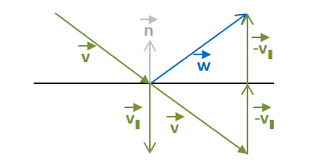
\includegraphics[scale=0.5]{images/Reflection.png}
\end{center}
The horizontal line in the figure represent a plane $\pi$ while $\underline{n}$ is its normal vector of length 1. 
Given $\underline{v}$ to obtain $\underline{w}$ we can use the following formula:
\[
\underline{w} = \underline{v} - 2(\underline{v}^\intercal \underline{n})\underline{n} = \underbrace{(I - 2\underline{n}\underline{n}^\intercal)}_{\text{reflection matrix}}\underline{v}
\]
Moreover, the reflection matrix $R$ is not only orthogonal, but also the inverse of itself, i.e. $R^{-1} = R^\intercal$. This makes sense because if we apply the reflection matrix twice, we obtain the original vector $\underline{v}$, i.e. the reflection of the reflection is the starting vector.

If we didn't have the 2 in the formula, we would obtain the projection of $\underline{v}$ on the plane $\pi$ which is called orthogonal projection and the matrix $R$ would be singular. \\

Let's now dive a bit into the third point of the factorization list. We said that when $S = S^\intercal$ (symmetric matrix) we can factorize it as $S = Q\Lambda Q^\intercal$ where $\Lambda$ is a diagonal matrix and $Q$ is an orthogonal matrix.\\
\[
S = S^\intercal = \underbrace{(Q\Lambda))}_{\tilde{Q}}Q^\intercal = \tilde{Q}Q^\intercal   
\]
\[
\tilde{Q} = \underline{q_1}\underline{\lambda_1} + \dots + \underline{q_n}\underline{\lambda_n}    
\]
Where the $q$ vectors are columns and $\lambda$ vectors are rows.
So we can reformulate:
\[
    S = (\underline{q_1}\underline{\lambda_1} + \dots + \underline{q_n}\underline{\lambda_n})Q^\intercal = \underline{q_1}\underline{\lambda_1}\underline{q_1}^\intercal + \dots + \underline{q_n}\underline{\lambda_n}\underline{q_n}^\intercal
\]
This is called \textbf{spectral decomposition} of matrix $S$ and $q_1, \dots, q_n$ are the eigenvectors of $S$ while $\lambda_1, \dots, \lambda_n$ are the eigenvalues of $S$.
\[
    S\underline{q_1} = \lambda_1\underline{q_1} = (\underline{q_1}\underline{\lambda_1}\underline{q_1}^\intercal + \dots + \underline{q_n}\underline{\lambda_n}\underline{q_n}^\intercal)\underline{q_1} = 
    \underline{\lambda_1}\underline{q_1}(\underline{q_1^\intercal}\underline{q_1})
    \]
All the other products are null since the vector $\underline{q_1}$ is orthogonal to all the other vectors $\underline{q_i}$ for $i \neq 1$ (recall that they are eigenvectors).

\section{Null spaces}
Let's consider the starting problem for a linear system of equations:
\[
A\underline{x} = \underline{b} \hspace{1cm} \text{with} \hspace{1cm} A\in \mathbb{R}^{m \times n}, \text{rank($A$)}=r    
\]

We are going to introduce 2 more spaces other than the column ones. To do so we consider:
\[
  A\underline{x} = \underline{0} \hspace{1cm} \rightarrow \hspace{1cm} N(A) \equiv \ker(A) = \{\underline{x} \in \mathbb{R}^n : A\underline{x} = \underline{0}\}  
\]
\[
    A^\intercal\underline{x} = \underline{0} \hspace{1cm} \rightarrow \hspace{1cm} N(A^\intercal) \equiv \ker(A^\intercal) = \{\underline{x} \in \mathbb{R}^n : A^\intercal\underline{x} = \underline{0}\}    
\]

So now, adding the so called \textbf{null spaces} we have that:
\begin{enumerate}
    \item $\mathcal{C}(A) \subset  \mathbb{R}^m$ and $dim(\mathcal{C}(A)) = r$
    \item $\mathcal{C}(A^\intercal) \subset \mathbb{R}^n$ and $dim(\mathcal{C}(A^\intercal)) = r$
    \item $N(A) \subset \mathbb{R}^n$ and $dim(N(A)) = ?$
    \item $N(A^\intercal) \subset \mathbb{R}^m$ and $dim(N(A^\intercal)) = ?$
\end{enumerate}
We still do not know the dimensions of those spaces. \\

\textbf{Example}\\
\[
A = \begin{bmatrix}
    1 & 4 & 7\\
    2 & 5 & 8\\
    3 & 6 & 9
\end{bmatrix}
\begin{bmatrix}
    x_1\\
    x_2\\
    x_3
\end{bmatrix}
= 
\begin{bmatrix}
    0\\
    0\\
    0
\end{bmatrix}
\hspace{0.3cm} \implies \hspace{0.3cm}
\begin{cases}
    x_1 + 4x_2 + 7x_3 = 0\\
    2x_1 + 5x_2 + 8x_3 = 0\\
    3x_1 + 6x_2 + 9x_3 = 0
\end{cases}    
\]
We compute the first equation
\[
    x_1 = -4x_2 - 7x_3 \hspace{0.3cm} \implies \hspace{0.3cm} \begin{cases}
        -3x_2 - 6x_3 = 0\\
        -6x_2 - 12x_3 = 0
    \end{cases}
\]
What is important to notice is that $A$ has rank$=2$ so we have $3-2=1$  \textbf{degrees of freedom}, i.e. we can choose one variable and the other two are automatically defined. This is visible in the last two equations of the system for example. 
In general, the degrees of freedom are given by $n-r$ where $n$ is the number of columns of $A$ and $r$ is the rank of $A$.\\

If we had 10 instead of 9 in $A$ we would have had $3-3=0$ degrees of freedom. This would translate in having the matrix $A$ full rank and $N(A) = \{\underline{0}\}$ so the only solution would be the null vector.


\section{Null space cardinality}
In the first lecture, we defined 4 spaces: $N(A), N(A^\intercal), \mathcal{C}(A), \mathcal{C}(A^\intercal)$. For the last two we defined also their cardinality whilst for the first ones we weren't able to tell yet. In this lecture we are going to find those values and prove them. In order to do so, we start from few useful properties:
\begin{enumerate}
    \item $\underline{x} = \underline{0} \in N(A)$ for any matrix $A$
    \item if $\underline{x}, \underline{y} \in N(A) \implies A(\underline{x} + \underline{y}) = \underline{0}$
    \item if $\underline{x} \in N(A) \implies \alpha\underline{x}$ with $\alpha \in \mathbb{R} \implies A(\alpha\underline{x}) = \underline{0}$
\end{enumerate}  

Consider, once again, the matrix $A \in \mathbb{R}^{m\times n}$, rank($A$) = $r \leq n$. 
We have seen the decomposition $A = CR$, where $C$ contains the linearly independent columns of $A$ and $R$ contains the coefficients that allow to recover the columns of $A$ starting from its independent columns. 
So, the matrix $A$ can be rewritten as:
\[
  A = \begin{bmatrix}
    A_1 & A_2
  \end{bmatrix} 
  \hspace{1cm}
  A_1 \in \mathbb{R}^{m\times r} \hspace{1cm} A_2 \in \mathbb{R}^{m\times (n-r)} 
\]
Where $A_1$ contains the independent columns of $A$ and $A_2$ the dependent ones.
Example:
\[
A = 
\begin{bmatrix}
    1 & 4 & 7\\
    2 & 5 & 8\\
    3 & 6 & 9
\end{bmatrix}
= 
\underbrace{
\begin{bmatrix}
1 & 4\\
2 & 5\\
3 & 6
\end{bmatrix}}_{A_1}
\begin{bmatrix}
    1 & 0 & -1\\
    0 & 1 & \undermat{B}{2}
\end{bmatrix}
\]
Since we have the last column of $A$, that is linearly dependent so it belongs to $A_2$, we can reformulate it in this way:
\[
    A = \begin{bmatrix}
        A_1 & A_2
      \end{bmatrix} 
    = \begin{bmatrix}
        A_1 & A_1B
    \end{bmatrix}
\]
We build a new matrix $K$ defined as follows:
\[
    K = \begin{bmatrix}
        -B\\
        I_{n-r}
    \end{bmatrix}
    \hspace{1cm}
    K \in \mathbb{R}^{n\times(n-r)}    
    \hspace{1cm}
    B \in \mathbb{R}^{r\times(n-r)}    
\]

\[
AK = \begin{bmatrix}
    A_1 & A_1B
\end{bmatrix} 
\begin{bmatrix}
    -B\\
    I_{n-r}
\end{bmatrix}
= A_1(-B) + A_1B = 0   
\]
Where the last 0 is actually a matrix of zeros of dimension $m\times(n-r)$
because A has size $m\times n$ and $K$ has size $n\times(n-r)$.
We have that:
\[
    AK = 0 \implies A\underline{k_i} = 0 \hspace{1cm} \forall i \in \{1, \dots, n-r\}    
\]
Where $k_i$ is the i-th column of $K$. This means that: $\underline{k_i} \in N(A) \hspace{0.2cm} \forall i$.

Now, we want to demonstrate that: $K\underline{u} = 0 \implies \underline{u} = \underline{0}$. 
To do so, we start from expanding $K$ from its definition:
\[
    K = \begin{bmatrix}
        -B\\
        I
    \end{bmatrix}
    \underline{u} = 0
    \implies
    \begin{bmatrix}
        -B\underline{u}\\
        \underline{u}
    \end{bmatrix}
    = 
    \begin{bmatrix}
        \underline{0}\\
        \underline{0}
    \end{bmatrix}
\]
Where the two zero vectors have dimension $r$ and $n-r$ respectively! Considering the second row of the matrix we get: $\underline{u} = \underline{0}$ so all columns of $K$ are linearly independent.\\

If we consider the problem ($\star$) $A\underline{x} = \underline{0}$, we want to prove that each \underline{x} that satisfy ($\star$) must be a linear combination of the columns of $K$.\\
\[
    A_1\underline{x} = \underline{0} \in \mathbb{R}^m \implies \underline{x} = \underline{0} \in \mathbb{R}^r    
\]
Because $A_1$ has linearly independent columns, i.e. has full rank.
\[
    A\underline{u} = \underline{0} \in \mathbb{R}^m \implies \begin{bmatrix}
        A_1 & A_1B
    \end{bmatrix} 
    \begin{bmatrix}
        \underline{u_1}\\
        \underline{u_2}
    \end{bmatrix}  
    = 
    \begin{bmatrix}
        A_1\underline{u_1} + A_1B\underline{u_2}\\
    \end{bmatrix}
    = 
    A_1\left[\underline{u_1} + B\underline{u_2}\right]
    = \underline{0}
\]
We can notice that the last formulation obtained in the equation has the same form as the one from where we started the prove, so we can say that:
\[
    \underline{u_1} + B\underline{u_2} = \underline{0} \implies \underline{u_1} = -B\underline{u_2}    
\]
\[
   \underline{u} = \begin{bmatrix}
    -B\underline{u_2}\\
    \underline{u_2}
\end{bmatrix}
    =
\underbrace{\begin{bmatrix}
    -B\\
    I
\end{bmatrix}}_{K}
    \underline{u_2}
    = K\underline{u_2}
    \implies 
    dim(N(A)) = n - r
\]


\begin{center}
    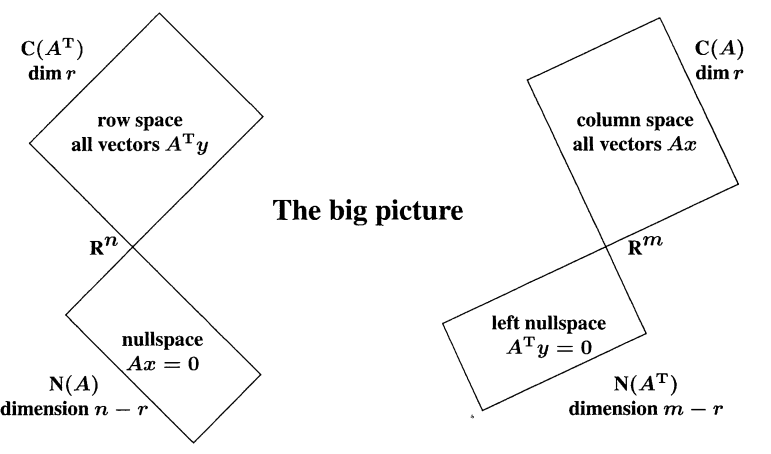
\includegraphics[scale = 0.4]{../images/SpacesDimensions.png}
\end{center}


\section{Eigenvalues and eigenvectors}
Start considering a generic square matrix $n \times n$. We are going later to discuss even the simmetry and positive definite properties.
Here below are the vectorial and the matrix form of the eigenvalue problem:
\[
    A\underline{x_i} = \lambda_i\underline{x_i} \hspace{0.5cm} i = 1, \dots, n \hspace{1cm} X^{-1}AX = \Lambda
\]
Where in the right-hand side there is a diagonal matrix $\Lambda$ with the eigenvalues of $A$ on the diagonal while the matrix $X$ with the eigenvectors of $A$ as columns.\\

\subsection{Eigenvectors of matrix power}
What can we say about the eigenvectors and eigenvalues of $A^2$?
\[
    A^2\underline{x_i} = A(A\underline{x_i}) = A(\lambda_i\underline{x_i}) = \lambda_i(A\underline{x_i}) = \lambda_i^2\underline{x_i}    
\]
So the eigenvalues of $A^2$ are the eigenvalues of $A$ squared.This is valid for any power of $A$ since this method can be applied recursively and it is very useful when there are problems in which a matrix is iteratively multiplied many times. \\

\textbf{Important}:\\
Given $A\in \mathbb{R}^{n\times n}$ full rank, then any vector $\underline{v} \in \mathbb{R}^n$ can be written as a linear combination of the eigenvectors ($x_i$) of $A$.\\

\subsection{Power method}
In mathematics, power iteration (also known as the power method) is an eigenvalue algorithm: given a diagonalizable matrix A, the algorithm will produce a number $\lambda$ , which is the greatest (in absolute value) eigenvalue of A, and a nonzero vector v, which is a corresponding eigenvector of $\lambda$ , that is, $Av=\lambda v$. The algorithm is also known as the Von Mises iteration.

There is also an \textbf{inverse PM} which is applied to $A^{-1}$ to find the minimum eigenvalue or also \textbf{PM with a shift} applied to $(A-\alpha I)^{-1}, \alpha \in \mathbb{R}$ to find the closest eigenvalue to $\alpha$. 

Can even be used in "deflation method" iteratively:
\[
    \begin{bmatrix}
        \lambda_1 & \underline{b_1^\intercal}\\
        0 & A_1
    \end{bmatrix}    
\]
the original matrix could be reduced in that form and at every iteration the procedure is applied to the $A_1$ matrix. This works only if we have different eigenvectors (or values) [check].

\subsection{Similar matrices}
Given two matrices $A, B \in \mathbb{R}^n$, they are said to be similar if $B = M^{-1}AM$, with $M$ invertible. 
\[
    \underbrace{M^{-1}AM}_{B}\underline{y} = \lambda \underline{y} \implies A\underbrace{M\underline{y}}_{\underline{w}} = \lambda \underbrace{M\underline{y}}_{\underline{w}} = A\underline{w} = \lambda \underline{w}    
\]
Where $\lambda, \underline{y}$ contain respectively the eigenvalues and the eigenvectors of $B$. What we get from this equation is that \textbf{similar matrices share the same eigenvectors with scaled eigenvalues}.

\subsection{QR factorization}
Here is introduced in the context of eigenvalues. Let's consider a matrix $A \in \mathbb{R}^{m\times n}$ where $m \geq n$ and $rank(A) = n$ (it has all independent columns). We can factorize $A$ in this way:
\[
    A = QR \hspace{1cm} Q \in \mathbb{R}^{m\times n} \hspace{1cm} R \in \mathbb{R}^{n\times n}
\]
Where is $Q$ is an orthogonal matrix and $R$ is an upper triangular matrix.Since we are dealing with eigenvalues and eigenvectors, we are now going to consider the matrix $A$ squared with the dimension $n\times n$.

\subsubsection{QR iteration} 
\[
    A = A^{(0)} = Q^{(0)}R^{(0)}     
\]
\[
    A^{(1)} = {Q^{(0)}}^{\intercal} A^{(0)} Q^{(0)} = Q^{(1)} R^{(1)}    
\]
So, iterating this procedure we get:
\[
    A^{(2)}, \dots, A^{(S)} = \text{is upper triangular}
\]
After S iterations you obtain an upper triangular matrix. The matrices $A, A^{(0)}, A^{(1)}, \dots, A^{(S)}$ are similar, so they share the same eigenvalues.

But, how can i compute $Q$?\\
With the \textbf{Gram-Schmidt} procedure. It works also for non-square matrices.\\
Let's start from a generic matrix $A$:
\[
    A = \begin{bmatrix}
        \vline & \vline & \vline\\
        \underline{a_1} & \ldots & \underline{a_n}\\
        \vline & \vline & \vline
    \end{bmatrix} 
\]
The algorithm is iterative and it is applied to the columns of $A$ in such way:
\[
  \underline{q_1} = \frac{\underline{a_1}}{||\underline{a_1}||}  
\]
The vector $\underline{q_1}$ is obtained by normalizing the first column of $A$, in such manner the new obtained vector will have norm 1.
\[
    \underline{q_2} = \underline{a_2} - \underline{q_1}(\underline{q_1}^\intercal \underline{a_2}) \implies \underline{q_2} = \dfrac{\underline{q_2}}{||\underline{q_2}||}
\]
The second vector is obtained by subtracting from the second column of $A$ the projection of $\underline{a_2}$ on $\underline{q_1}$, in such manner the new vector will be orthogonal to $\underline{q_1}$ and will have norm 1.
\[
    \underline{q_3} = \underline{a_3} - \underline{q_1}(\underline{q_1}^\intercal \underline{a_3}) - \underline{q_2}(\underline{q_2}^\intercal \underline{a_3}) \implies \underline{q_3} = \dfrac{\underline{q_3}}{||\underline{q_3}||}
\]
And so on... Recall that the orthogonality is needed since we want to obtain an orthogonal matrix $Q$ useful for the factorization. With Gram-Schmidt the resulting matrix not only will be orthogonal but also orthonormal, this means that its columns will have norm unitary.\\  
Let's now continue with the factorization journey. We have said in the introduction of types of factorizations that, given $A \in \mathbb{R}^{n\times n}$, we have:
\[
    A = X \Lambda X^{-1}
\]
Where $X$ has as columns the eigenvectors of A, while $\Lambda$ is a diagonal matrix with the eigenvalues of $A$ on the diagonal. Now, let's consider the case where the matrix $S$ is symmetric.
\[
    S \in \mathbb{R}^{n\times n} \hspace{1cm} S = S^\intercal
\]
We can factorize $S$ as follows:
\[
    S = Q \Lambda Q^\intercal
\]
Where $Q$ is orthogonal (this is true only because $S$ is symmtric) and $\Lambda$ is diagonal.
We can prove that $Q$ is orthogonal by:
\begin{enumerate}
    \item Consider the two vectors $\underline{x}, \underline{y}$ such as: $S\underline{x} = \lambda\underline{x}$ and $S\underline{y} = 0\underline{y}$. So, we are saying that both vectors are eigenvectors.
    \[
        \begin{rcases}
            \underline{y} \in N(S)\\
            \underline{x} \in \mathcal{C}(S) = \mathcal{C}(S^{\intercal})    
        \end{rcases}
        \implies \underline{x} \perp \underline{y}
    \]
    This is confirmed also by the scheme done during lecture with the 4 blocks. Notice that we have not specified or made any assumption on the value of $\lambda$.
    \item Similar to point 1, we consider the two vectors $\underline{x}, \underline{y}$ such as: $S\underline{x} = \lambda\underline{x}$ and $S\underline{y} = \alpha\underline{y}$. Now, consider the matrix $(S - \alpha I)$, we can write:
    \[
        (S - \alpha I)\underline{y} = 0\underline{y} \implies \underline{y} \in N(S - \alpha I)
    \]
    \[
        (S - \alpha I)\underline{x} = (\lambda - \alpha)\underline{x} \implies \underline{x} \in \mathcal{C}(S - \alpha I) = \mathcal{C}((S - \alpha I)^{\intercal})
    \]
    So, again we obtain: $\underline{x} \perp \underline{y}$.
\end{enumerate}
There is another property: $\lambda_i \in \mathbb{R}$, so the eigenvalues on the diagonal of $\Lambda$ are real. Proof:
\[
    S\underline{x} = \lambda\underline{x} \implies \overline{\underline{x}}^\intercal S\underline{x} = \lambda\overline{\underline{x}}^\intercal\underline{x}     
\]
The $\overline{\underline{x}}$ represent the conjugate of the vector $\underline{x}$. If that vector has complex components, those elements are conjugated, otherwise, i.e. they are all real, they remain inalterated. In particular, once a complex number is conjugated, the result is a real number, as shown here:
\[
    (a + ib)(a - ib) = (a^2 + b^2) \in \mathbb{R}    
\]
From the previos equation, we obtain:
\[
    \lambda = \frac{\overline{\underline{x}}^\intercal S\underline{x}}{\overline{\underline{x}}^\intercal\underline{x}} \in \mathbb{R}
\]

\subsection{Positive-definite symmetric matrices (SPD)}
Characterizations:
\begin{enumerate}[i]
    \item $\lambda_i > 0 \hspace{0.5cm} \forall i = 1, \dots, n$
    \item $\underline{v}^\intercal S \underline{v} \geq 0 \hspace{0.5cm} \forall \underline{v} \in \mathbb{R}^n$, with equality if and only if $\underline{v} = 0$
    \item Leading determinants are positive. \\
    \begin{multicols}{2}
        \begin{center}
            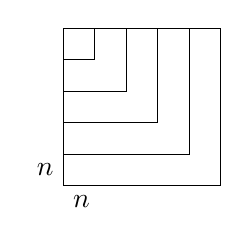
\begin{tikzpicture}
                \draw (0,0) -- (2,0) -- (2,2) -- (0,2) -- (0,0);
                \draw (0,0.4) -- (1.6,0.4) -- (1.6,2) -- (0,2) -- (0,0);
                \draw (0,0.8) -- (1.2,0.8) -- (1.2,2) -- (0,2) -- (0,0); 
                \draw (0,1.2) -- (0.8,1.2) -- (0.8,2) -- (0,2) -- (0,0) node[above left]{$n$};
                \draw (0,1.6) -- (0.4,1.6) -- (0.4,2) -- (0,2) -- (0,0) node[below right]{$n$};
            \end{tikzpicture}
        \end{center}

        This means that the determinant of the matrix obtained by taking the first $k$ rows and columns of $S$ is positive, $\forall k = 1, \dots, n$.
    \end{multicols}

    \item Cholesky decomposition: $S = B^\intercal B$, with $B$ upper triangular
    \item All pivot elements are positive in the Gaussian elimination process
\end{enumerate}

Let's consider $\lambda > 0$ being a certain eigenvalue. 
\[ 
    S\underline{x} = \lambda\underline{x}    
\]
We multiply both sides by $\underline{x}^\intercal$:
\[
    \underline{x}^\intercal S\underline{x} = \lambda\underline{x}^\intercal\underline{x} = \lambda\||\underline{x}\||^2 \geq 0
\]
Recall that $\underline{x}$ is an eigenvector while the before considered vector $\underline{v}$ is a generic vector. With $\underline{v}$, instead, we have:
\[
    \underline{v} = (c_1\underline{x}_1 + c_2\underline{x}_2 + \dots + c_n\underline{x}_n)    
\]
So we are expressing $\underline{v}$ as a linear combination of the eigenvectors of $S$. 
\[
    (c_1\underline{x}_1 + c_2\underline{x}_2 + \dots + c_n\underline{x}_n)^\intercal S (c_1\underline{x}_1 + c_2\underline{x}_2 + \dots + c_n\underline{x}_n)        
\]
\[
    \begin{rcases}
        c_1^2\underline{x}_1^\intercal S \underline{x}_1 = c_1^2\lambda_1\underline{x}_1^\intercal \underline{x}_1 = c_1^2\lambda_1||\underline{x}_1||^2\\
        c_1c_2\underline{x}_1^\intercal S \underline{x}_2 = c_1c_2\lambda_2\underline{x}_1^\intercal \underline{x}_2 = 0\\
    \end{rcases}    
    \text{there are two types of components}
\]
The first components is given by the eigenvectors with the same direction, while the second no so their scalar product is null (they are orthogonal).\\

From \textit{iv}):
\[
    S = B^\intercal B \implies \underline{v}^\intercal(B^\intercal B)\underline{v} = (\underline{v}^\intercal B^\intercal)(B \underline{v}) = (B\underline{v})^\intercal (B\underline{v}) = ||B\underline{v}||^2 \geq 0   
\]

\section{Singular Value Decomposition (SVD)}
We are going to use it for:
\begin{itemize}
    \item Least-squares approximation by introducing the pseudo-inverse of a matrix (Moore-Penrose inverse)
    \item Low-rank approximation with the Eckart-Young theorem
\end{itemize}
We start from:
\[
A \in \mathbb{R}^{m \times n} \hspace{1cm} 
\begin{cases}
m = \text{\# of samples}\\
n = \text{\# of features}
\end{cases}    
\]
We can write:
\[
    A = U\Sigma V^\intercal    
\]
With:
\begin{itemize}
    \item $U$ with dimensions $m \times m$ and orthogonal
    \item $\Sigma$ with dimensions $m \times n$ \textit{almost} diagonal
    \item $V^\intercal$ with dimensions $n \times n$ and orthogonal
\end{itemize}
If $m > n$, we can represent the matrices like this:
\[
\underbrace{
  \begin{bmatrix}
    & & & & & \\
    & & & & & \\
    & & & & & \\
    & & & & & \\
    & & & & & \\
  \end{bmatrix}}_{m \times m}
\underbrace{
  \begin{bmatrix}
    & & & \\
    & & & \\
    & & & \\
    & & & \\
    & & & \\
  \end{bmatrix}}_{m \times n}
\underbrace{
  \begin{bmatrix}
    & & & \\
    & & & \\
    & & & \\
  \end{bmatrix}}_{n \times n}
\]
What is the idea of SVD? Try to change features so variances are maximized and covariances are minimized. We don't want columns to be correlated.\\

In general: rank($A$) = $r < n$.
\[
    AV = U\Sigma \impliedby V^\intercal V = I \impliedby V \text{ is orthogonal}    
\]
The component wise notation is:
\[
    A\underline{v_i} = \sigma_i\underline{u_i}    
\]
Given that the rank of $A$ is $r$:

\[
\begin{bmatrix}
    & & & & & & &\\
    & & & & & & &\\
    & & & & & & &\\
    & & & & & & &\\
    & & & & & & &\\
    & & & & & & &\\
\end{bmatrix}
\begin{bmatrix}
    \sigma_1 & & & &\\
    & \sigma_2 & & &\\
    & & \ddots & &\\
    & & & \sigma_r &\\
    & & & & 0\\
    \hline
    0 & 0 & 0 & 0 & 0\\
    0 & 0 & 0 & 0 & 0\\
\end{bmatrix}
\begin{bmatrix}
    & & & & \\
    & & & & \\
    & & & & \\
    & & & & \\
\end{bmatrix}
\hspace{1cm}
\begin{cases}
\sigma_1, \dots, \sigma_r > 0\\
\sigma_{r+1}, \dots, \sigma_n = 0
\end{cases}  
\]
Typically: $\sigma_1 > \sigma_2 > \dots > \sigma_r > \sigma_{r+1} = 0$.
We have:
\[
\begin{cases}
    \begin{rcases}
        A\underline{v_1} = \sigma_1\underline{u_1}\\
        \hspace{1cm}\vdots\\
        A\underline{v_r} = \sigma_r\underline{u_r}\\        
    \end{rcases} r\\
    \begin{rcases}
        A\underline{v_{r+1}} = \sigma_{r+1}\underline{u_{r+1}}\\
        \hspace{1cm}\vdots\\
        A\underline{v_n} = \sigma_n\underline{u_n}\\        
    \end{rcases} n-r
\end{cases}    
\]
So the first $r$ vectors span the column space of $A$ while for the last $n-r$ means that $\underline{v_i} \in N(A)$ for $i = r+1, \dots, n$.
If we have $A^\intercal$, the decomposition is $A^\intercal = (U\Sigma V^\intercal)^\intercal = V\Sigma^\intercal U^\intercal$. 

\subsection{Economy SVD}
What we've seen so far is the full SVD, but it can be optimized. Here is following the compact (reduced) representation, where once again we consider $m > n$:
\[
\underbrace{
  \begin{bmatrix}
    & & & \\
    & & & \\
    & & & \\
    & & & \\
    & & & \\
  \end{bmatrix}}_{m \times n}
\underbrace{
  \begin{bmatrix}
    & & & \\
    & & & \\
    & & & \\
  \end{bmatrix}}_{n \times n}
\underbrace{
  \begin{bmatrix}
    & & & \\
    & & & \\
    & & & \\
  \end{bmatrix}}_{n \times n}
\]
This is caused by the fact that the last $m-n$ rows in the central matrix are all 0 so multiply them for the last $m-n$ columns of the left matrix is useless. This can be furthermore optimized by having matrix dimensions: $(m\times r)(r\times r)(r\times n)$ because not all $\sigma$ might be different than 0 (i.e. the rank of $A$ is $r$), so, in that case is useless even to multiply the last $m-r$ rows of the central matrix. \\

\textbf{The SVD works for any matrix $A$.}\\

\noindent Let's suppose $A$ is full rank $n\times n$:
\[
    A = U\Sigma V^\intercal = \sum_{i = 1}^{n} \sigma_i \underbrace{\underline{u_i}\underline{v_i}^\intercal}_{\text{rank }=1}    
\]
View matrix-matrix multiplication for the rank 1 concept.
If $A$ is not full rank but instead has rank($A$)=$r$, the same sum is nomore computed until $n$, but instead $r$.
\[
    A = \sum_{i = 1}^{r} \sigma_i \underline{u_i}\underline{v_i}^\intercal   
\]
What happens now if we pick a certain value $\tilde{r} < r$?
\[
    A = U\Sigma V^\intercal \cong \sum_{i = 1}^{\tilde{r}} \sigma_i \underline{u_i}\underline{v_i}^\intercal   
\]
We obtain a \textbf{rank $\tilde{r}$ approximation of the matrix A}. The rank of the matrix is know because is the sum of $\tilde{r}$ matrices of rank 1. Moreover, that one, is the best approximation of rank $\tilde{r}$ possible, i.e.:
\[
    ||A - \tilde{A}|| \leq ||A - B|| \hspace{1cm} \forall B  \text{ of rank} = \tilde{r}    
\]

\subsection{Proof of the existence of SVD}
Once again, we start from matrix $A \in \mathbb{m \times n}$ an rank$=r$. We consider the new matrix $A^\intercal A$ which is:
\begin{itemize}
    \item symmetric: $(A^\intercal A)^\intercal = A^\intercal A$
    \item positive definite: $\underline{x}^\intercal(A^\intercal A)\underline{x} = (\underline{x}^\intercal A^\intercal)(A \underline{x}) = (A\underline{x})^\intercal (A\underline{x}) = ||A\underline{x}||^2 \geq 0  $
\end{itemize} 
We can use the following decomposition:
\[
    A^\intercal A = V\Lambda V^\intercal = \sum_{i=1}^n \lambda_i \underline{v_i} \underline{v_i^\intercal}    
\]
Recall that $V$ contains the eigenvectors while $\Lambda$ contains the eigenvalues. We rename $\lambda_i = \sigma_i^2$. The rank of $A^\intercal A$ is $r$.\\

We want to prove that if  $\underline{x} \in N(A)$ then $\underline{x} \in N(A^\intercal A)$, to do so we proceed in both directions:
\begin{enumerate}
    \item If we have $A\underline{x} = 0 \implies \underline{x} \in N(A)$. Is it possible to multiply both terms:
    \[
        A^\intercal(A\underline{x}) = A^\intercal \underline{0} = \underline{0} \hspace{1cm} \text{so} \hspace{1cm} \underline{x} \in N(A) \implies \underline{x} \in N(A^\intercal A)
    \]
    \item We start from $(A^\intercal A)\underline{x} = 0 \implies \underline{x} \in N(A^\intercal A)$. Again, we multiply:
    \[
        \underline{x}^\intercal A^\intercal A\underline{x} = ||A\underline{x}||^2 = 0 \hspace{1cm} \text{so} \hspace{1cm} \underline{x} \in N(A^\intercal A) \implies \underline{x} \in N(A)
    \]
\end{enumerate}
Let's consider the couple of (eigenvalues, eigenvectors) = ($\sigma_i^2, \underline{v_i}$):
\[
    A^\intercal A\underline{v_i} = \sigma_i^2 \underline{v_i} \hspace{0.3cm}\overset{\text{component-wise}}{\longrightarrow} \hspace{0.3cm} A^\intercal A\underline{v_i} = \sigma_i^2 \underline{v_i} \hspace{1cm} (\dagger)
\]
We introduce the quantity $\underline{u_i} = \dfrac{A\underline{v_i}}{\sigma_i}$ which has some characteristics:
\begin{enumerate}[i]
    \item $\underline{u_i}$ are unitary vectors:
    \[
        \underline{u_i}^\intercal \underline{u_i} = \left(\dfrac{A\underline{v_i}}{\sigma_i}\right)^\intercal \left(\dfrac{A\underline{v_i}}{\sigma_i}\right) = \dfrac{\underline{v_i^\intercal}A^\intercal A\underline{v_i}}{\sigma^2} \overset{\dagger}{=} \dfrac{\sigma_i^2 \underline{v_i^\intercal}\underline{v_i}}{\sigma_i^2} = 1
    \]
    The last passage of the equation is true because $\underline{v_i}$ vectors are orthonormal.
    \item $\underline{u_i} \perp \underline{u_j}$:
    \[
        \underline{u_i}^\intercal \underline{u_j} = \left(\dfrac{A\underline{v_i}}{\sigma_i}\right)^\intercal \left(\dfrac{A\underline{v_j}}{\sigma_j}\right) = \dfrac{\underline{v_i^\intercal}A^\intercal A\underline{v_j}}{\sigma_i \sigma_j} \overset{\dagger}{=} \dfrac{\sigma_j^2 \underline{v_i^\intercal}\underline{v_j}}{\sigma_i \sigma_j} = 0
    \] 
    \item $\underline{u_i}$ are eigenvectors of $AA^\intercal$ with eigenvalues $\sigma_i^2$:
    \[
        (AA^\intercal \underline{u_i}) = AA^\intercal\left(\dfrac{A\underline{v_i}}{\sigma_i}\right) = A\dfrac{A^\intercal A\underline{v_i}}{\sigma_i} \overset{\dagger}{=} A\dfrac{\sigma_i^2 \underline{v_i}}{\sigma_i} = \sigma_i^2\left(\dfrac{A\underline{v_i}}{\sigma_i}\right) = \sigma_i^2\underline{u_i}   
    \]
\end{enumerate}
We have demonstrated that $A\underline{u_i} = \sigma_i \underline{u_i}$ and $\underline{u_i}$ are orthonormal as well. 
We have seen that $\underline{u_i} = \frac{A\underline{v_i}}{\sigma_i}$ but, what happen if $\sigma_i = 0$?\\
Until now we have assumed that could not happen. Let's 2 examples, in the first we have the standard case while in the second is explained how to manage the case $\sigma_i = 0$.\\

\textbf{Example 1}
\[
A = \begin{bmatrix}
    4 & 4\\
    -3 & 3\\
\end{bmatrix} \hspace{1cm} \text{rank}(A) = 2
\]
We build two new matrices $X$ and $Y$:
\[
X = A^\intercal A = \begin{bmatrix}
    25 & 7\\
    7 & 25\\
\end{bmatrix} \hspace{1cm} \text{eigs}(X) = 
\begin{cases}
    \lambda_1 = 18 \hspace{1cm} \underline{v_1} = \begin{bmatrix}
        -\frac{\sqrt{2}}{2}\\
        \frac{\sqrt{2}}{2}\\
    \end{bmatrix}\\
    \lambda_2 = 32 \hspace{1cm} \underline{v_2} = \begin{bmatrix}
        \frac{\sqrt{2}}{2}\\
        \frac{\sqrt{2}}{2}\\
    \end{bmatrix}\\
\end{cases}    
\]
\[
Y = AA^\intercal = \begin{bmatrix}
    32 & 0\\
    0 & 18\\
\end{bmatrix} \hspace{1cm} \text{eigs}(Y) =
\begin{cases}
    \lambda_1 = 18 \hspace{1cm} \underline{u_1} = \begin{bmatrix}
        1\\
        0\\
    \end{bmatrix}\\
    \lambda_2 = 32 \hspace{1cm} \underline{u_2} = \begin{bmatrix}
        0\\
        1\\
    \end{bmatrix}\\
\end{cases}    
\]
So we have all elements for contructing the SVD:
\[
U = 
\begin{bmatrix}
    0 & 1\\
    1 & 0\\
\end{bmatrix}
\hspace{1cm}
\Sigma =
\begin{bmatrix}
    \sqrt{18} & 0\\
    0 & \sqrt{32}\\
\end{bmatrix}    
\hspace{1cm}
V =
\begin{bmatrix}
    -\frac{\sqrt{2}}{2} & \frac{\sqrt{2}}{2}\\
    \frac{\sqrt{2}}{2} & \frac{\sqrt{2}}{2}\\
\end{bmatrix}
\]
It is easy to verify that $A = U\Sigma V^\intercal$.

\textbf{Example 2}
\[
A = \begin{bmatrix}
    4 & 3\\
    8 & 6\\
\end{bmatrix}
\hspace{1cm}
\text{rank}(A) = 1    
\]\\
As in the example before, we start building our matrices $X$ and $Y$:
\[
X = A^\intercal A = \begin{bmatrix}
    80 & 60\\
    60 & 45\\
\end{bmatrix}
\hspace{1cm}
\text{eigs}(X) =
\begin{cases}
    \lambda_1 = 125 \hspace{1cm} \underline{v_1} = \begin{bmatrix}
        \frac{-4}{5}\\
        \frac{-3}{5}\\
    \end{bmatrix}\\
    \lambda_2 = 0 \hspace{1cm} \underline{v_2} = ?
\end{cases}
\]
How can we compute the value of $\underline{v_2}$? The idea is to bild a vector $\underline{v_2}$ such that it is orthogonal to $\underline{v_1}$. 
A possible solution is: $\underline{v_2} = \begin{bmatrix}
    \frac{3}{5}\\
    \frac{-4}{5}\\
\end{bmatrix}$.\\
The equation at the beginning of this page (the one regarding $\underline{u_i}$) can still be computed for the vector $\underline{v_1}$ in this case:
\[
\underline{u_1} = \dfrac{A\underline{v_1}}{\sigma_1} = \dfrac{1}{\sqrt{125}}\begin{bmatrix}
    4 & 3\\
    8 & 6\\
\end{bmatrix}
\begin{bmatrix}
    \frac{-4}{5}\\
    \frac{-3}{5}\\
\end{bmatrix} = \dfrac{1}{\sqrt{125}}\begin{bmatrix}
-5\\
-10\\    
\end{bmatrix}
\]
Now, the problem rises again because $\sigma_2 = 0$ so we cannot compute $\underline{u_2}$. In reality, we do not need to compute $\underline{u_2}$ because $\underline{u_1}$ and $\underline{v_1}$ are sufficient to recover the original matrix through (reduced) SVD, indeed:
\[
\underbrace{
\dfrac{1}{\sqrt{125}} \begin{bmatrix}
    -5 \\
    -10\\
\end{bmatrix}}_{U}
\underbrace{
\begin{bmatrix}
    \sqrt{125}
\end{bmatrix}}_{\Sigma}
\underbrace{ 
\begin{bmatrix}
    \frac{-4}{5} & \frac{-3}{5}\\
\end{bmatrix}}_{V}   
=
\begin{bmatrix}
    4 & 3\\
    8 & 6\\
\end{bmatrix}
\] 
We could have used also the full SVD with the following matrices:
\[
    U = \dfrac{1}{\sqrt{125}} \begin{bmatrix}
        -5 & -10\\
        -10 & 5\\
    \end{bmatrix}
\hspace{1cm}
\Sigma = \begin{bmatrix}
    \sqrt{125} & 0\\
    0 & 0\\
\end{bmatrix}
\hspace{1cm}
V = \begin{bmatrix}
    \frac{-4}{5} & \frac{-3}{5}\\
    \frac{-3}{5} & \frac{4}{5}\\
\end{bmatrix}
\]
Where $\underline{u_2}$ is the second column of the matrix $U$ and is a vector orthogonal to $\underline{u_1}$. All elements written here and not in the previous formulation are a waste of memory.
A concise recap of all versions of SVD:
\begin{enumerate}
    \item \textbf{full SVD}: $\underset{(m \times n)}{A} = \underset{(m \times m)}{U}\underset{(m \times n)}{\Sigma}\underset{(n \times n)}{V^\intercal}$
    \item \textbf{economy SVD}: $\underset{(m \times n)}{A} = \underset {(m \times n)}{U}\underset{(n \times n)}{\Sigma}\underset{(n \times n)}{V^\intercal}$
    \item \textbf{reduced SVD}: $\underset{(m \times n)}{A} = \underset{(m \times r)}{U}\underset{(r \times r)}{\Sigma}\underset{(r \times n)}{V^\intercal}$
    \item \textbf{truncated SVD approximation}: $\sum\limits_{i=1}^{\tilde{r}} \sigma_i\underline{u_i}\underline{v_i^\intercal}$
\end{enumerate}
For the first two cases the rank of $A$ is $n$, for the third is $r$ while in the first the approximation rank is decided.

\subsection{Geometrical interpretation of SVD}
Matrices $U, V^\intercal$ are orthonormal so, as mentioned in the section above, they represent a rotation (or reflection) while $\Sigma$, being a diagonal matrix, correspond to a scaling transformation. 
\begin{center}
    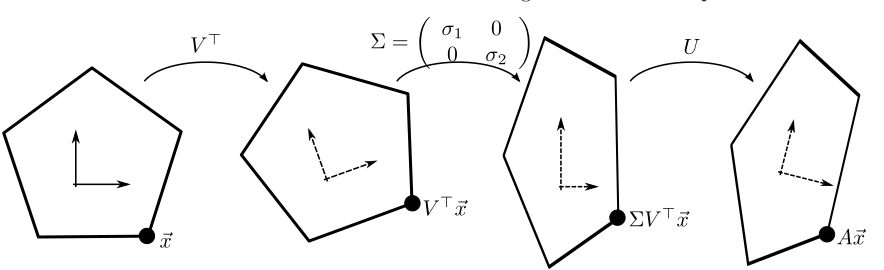
\includegraphics[scale=0.4]{../images/SVD_Geometric_Interpretation.png}
\end{center}
\textbf{Since for SVD no assumptions are made on the starting matrix, this means that \underline{any} matrix can be obtained from 2 rotations and 1 scaling.}\\

When $A$ is squared and symmetric ($A \in \mathbb{R}^{n\times n}, A=A^\intercal$)?

We can apply \textbf{polar decomposition}:
\[
A = QR    
\]
Where $Q$ is orthogonal and $S$ is symmetric positive semi-definite. Why? From SVD. 
\[
    A = U\Sigma V^\intercal = \underbrace{(UV^\intercal)}_{Q}\underbrace{(V\Sigma V^\intercal)}_{S}    
\]
In particular, the product of the two orthogonal matrices in the first parenthesis is always another orthogonal matrix. In this case of decomposition, matrix $A$ is obtained just by one rotation and one scaling (missing one more rotation with respect to classic SVD). Indeed, the second parenthesis results just in a stretch because $V$ and $V^intercal$ are two rotations identical and opposite, i.e. they cancels out. 

\subsubsection{Properties of SVD}
\begin{enumerate}[i]
    \item If A is orthogonal, then $\sigma_i = 1$ because if $A$ orthogonal then $A^\intercal A = I$
    \item All eigenvalues of a square matrix are $\leq \sigma_1$. Proof:
    \[
        ||A\underline{x}|| = ||U\Sigma V^\intercal \underline{x}|| = ||\Sigma V^\intercal \underline{x}|| \leq \sigma_1||V^\intercal \underline{x}|| = \sigma_1||\underline{x}|| \implies ||A\underline{x_i}|| \leq \sigma_1||\underline{x_i}||
    \]
    The matrix $U$ disappear becuase an orthogonal matrix, when multiplied, does not change the magnitude of a vector. If we consider
    \[
        ||A\underline{x_i}|| = ||\lambda_i\underline{x_i}|| = |\lambda_i|\cdot ||\underline{x_i}||
    \]
    \[
        |\lambda_i|\cdot ||\underline{x_i}|| \leq \sigma_1||\underline{x_i}|| \implies |\lambda_i| \leq \sigma_1 \hspace*{0.4cm} \forall i    
    \]
\end{enumerate}

\subsection{Snapshots method}
During real case scenarios, we will have a certain matrix $A \in \mathbb{m\times n}$ and it might happen that $m \gg n$ i.e. the number of samples is much greater than the number of features. In these cases, we can use the following trick to be more efficient.

For the SVD we need to compute both $AA^\intercal$ and $A^\intercal A$. Which one is better to start with? And why?
We would have $AA^\intercal: (m\times m)$ and $A^\intercal A: (n\times n)$. Given $m \gg n$ it is clear that the second one is better to start with becuase, being much smaller, it will be easier to computer its eigenvalues and eigenvectors.    


\subsection{Matrix norms}
This concept is an extension of the vector norm. Given a matrix $A \in \mathbb{R}^{m\times n}$, we define the matrix norm as:
\begin{itemize}
    \item \textbf{Frobenius norm}: $||A||_F = \sqrt{\sum\limits_{i=1}^{m}\sum\limits_{j=1}^{n}|a_{ij}|^2} = \sqrt{\Tr(A^\intercal A)} = \sqrt{\Tr(AA^\intercal)}$ \\
    Recall that $\Tr(AB) = \Tr(BA)$. \\
    Example:
    \[
        A = \begin{bmatrix}
            1 & 2\\
            3 & 4\\
            5 & 6\\
        \end{bmatrix} \hspace{1cm} ||A||_F = \sqrt{1^2 + 2^2 + 3^2 + 4^2 + 5^2 + 6^2} = \sqrt{91}
    \]
    \[
        \begin{bmatrix}
            1 & 2\\
            3 & 4\\
            5 & 6\\
        \end{bmatrix}
        \begin{bmatrix}
            1 & 3 & 5\\
            2 & 4 & 6\\
        \end{bmatrix} =
        \begin{bmatrix}
            1^2+2^2 & \hdots & \hdots\\
            \hdots & 3^2+4^2 & \hdots\\
            \hdots & \hdots & 5^2+6^2\\
        \end{bmatrix}  \implies \sqrt{\Tr(AA^\intercal)} = \sqrt{91}    
    \]
    If $U$ is orthogonal, what happen to $||AU||^2_F$?
    \[
        ||AU||^2_F = \Tr((AU)^\intercal AU) = \Tr(U^\intercal A^\intercal AU) = \Tr(A^\intercal A\underbrace{UU^\intercal}_{I}) = \Tr(A^\intercal A) = ||A||^2_F    
    \]
    This means that the Frobenius norm is invariant with respect to orthogonal transformations ($\dag$). \\ 
    The Frobenius norm is also equal to $\left(\sqrt{\sum\limits_{i=1}^{r}\sigma_i^2}\right)$ where $r$ is the rank of $A$. Proof:
    \[
        ||A||_F = ||U\Sigma V^\intercal||_F \overset{\dag}{=} ||\Sigma||_F \triangleq  \Tr\sqrt{(\Sigma\Sigma^\intercal)} = \sqrt{\sum\limits_{i=1}^{r}\sigma_i^2}    
    \]
    \item \textbf{P-norms}: Recall the p-norm for vectors:
    \[
        \underline{p} \in \mathbb{R}^n \implies ||\underline{p}||_p = \left(\sum\limits_{i=1}^n |p_i|^p\right)^{\frac{1}{p}}    
    \]
    Given $A \in \mathbb{R}^{m\times n}$ we can define the p-norm for that matrix as:
    \[
        ||A||_p = \underset{\underline{x} \in \mathbb{R}^n}{\sup} \dfrac{||A\underline{x}||_p}{||\underline{x}||_p} = \underset{\underline{x} \in \mathbb{R}^n, \hspace{0.1cm} ||\underline{x}||_p}{\sup} ||A\underline{x}||_p
    \]
    If you choose $p=2$ you get the operator norm and $||A||_2 = \sigma_1$.
\end{itemize}

\subsection{Eckart-Young theorem}
Having defined the norms, we can now proceed with the proof of the \textbf{Eckart-Young theorem} which states:\\

\emph{For either $||\cdot||_F$, $||\cdot||_2$ we have:}
\[
    ||A - A_k|| \leq ||A - B|| \hspace{1cm} \forall B \text{ of rank } k
\]
\emph{where} $A_k = \sum\limits_{i=1}^k \sigma_i\underline{u_i}\underline{v_i}^\intercal$ \emph{i.e. is the SVD approximation of rank k of the matrix A. Depending on the chosen norm you get:}
\[
    ||A - A_k|| = \begin{cases}
        \sigma_{k+1} \text{ if } ||\cdot||_2 \text{considered}\\
        \left(\sum\limits_{i=1}^{r} \sigma_i^2\right)^{\frac{1}{2}} \text{ if } ||\cdot||_F \text{ considered}
    \end{cases}
\]
There will be 2 proofs, one for each type of norm. 

\subsubsection{Proof considering $||\cdot||_F$}
We start from the \textbf{Weyl inequality}:
\[
    \sigma_{i+j-1}(X+Y) = \sigma_i(X) + \sigma_j(Y)    
\]
Where a generic $\sigma_k(E)$ is the k-eiths singular value of the matrix $E$.  
We define 
\[
X = A_k - B \hspace{2cm} Y = B    
\]
So we have
\[
\sigma_{i+k}(A) \leq \sigma_i(A-B) + \underbrace{\sigma_{k+1}(B)}_{0}
\]
The last component has value of 0 because the matrix $B$ has rank equal to $k$.
\[
||A - A_k||_F^2 = \left(\sum\limits_{i=k+1}^r \sigma_i^2(A)\right) \overset{\text{shift}}{\overset{\downarrow}{=}} \left(\sum\limits_{i=1}^{r-k} \sigma_{i+k}^2(A)\right) \leq \left(\sum\limits_{i=1}^{r-k} \sigma_{i+k}^2(A - B)\right) \leq \left(\sum\limits_{i=1}^{\min(m,n)} \sigma_{i+k}^2(A-B)\right) = ||A-B||_F^2
\]
In particular, recall that $A = \sum\limits_{i=1}^{r} \sigma_i\underline{u_i}\underline{v_i^\intercal}$ and $A_k = \sum\limits_{i=1}^{k} \sigma_i\underline{u_i}\underline{v_i^\intercal}$. The theorem is proved just by picking the first and last components of the inequality written above. 



\subsubsection{Proof considering $||\cdot||_2$}
We are now going to prove the theorem with the last norm we did not use yet. Let's consider the matrix $B$ with dimensions $n \times d$ and rank($B$)=$k$. This means that:
\[
    N(B) \subset \mathbb{R}^d \hspace{1cm} dim(N(B)) = d-k     
\]
If we consider matrix $V$ of the SVD decomposition of $A$:
\[
    V_{k+1} = \underbrace{\begin{bmatrix}
        \vline & \vline & \vline\\
        \underline{v_1} & \ldots & \underline{v_{k+1}}\\
        \vline & \vline & \vline
    \end{bmatrix}}_{k+1 \text{cols}}
\]
Those are the $k+1$ columns of $V$.
\[
\mathcal{C}(V_{k+1}) \subset \mathbb{R}^d  \hspace{1cm} dim(\mathcal{C}(V_{k+1})) = k+1  
\]
By adding the previous information, we have:
\[
    dim(N(B)) + dim(\mathcal{C}(V_{k+1})) = d - k + k + 1 = d + 1 
\]
Since both spaces are subset of $\mathbb{R}^d$ and their summed dimensions are $d+1$ this means that the intersection of those spaces is not empty.\\ 
\begin{center}
    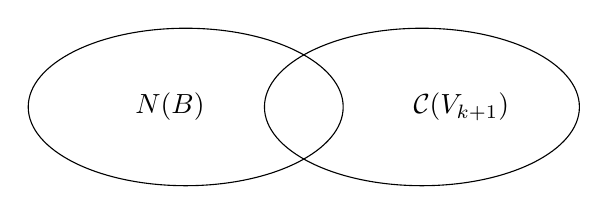
\begin{tikzpicture}
        \draw (0,0) ellipse (2cm and 1cm);
        \draw node at (-0.2,0) {$N(B)$};
        \draw (3,0) ellipse (2cm and 1cm);
        \draw node at (3.5,0) {$\mathcal{C}(V_{k+1})$};
    \end{tikzpicture}
\end{center}
Consider $\underline{w} \in N(B) \bigcap \mathcal{C}(V_{k+1})$, we suppose for easyness that $||\underline{w}||_2 = 1$.
\[
    \underline{w} = \sum_{i=1}^{k+1} c_i \underline{v_i} \overset{(\star)}{=} V_{k+1}\underline{c} \hspace{1cm} \sum_{i=1}^{k+1} c_i^2 = 1   
\]
We want to measure the following quantity:
\[
    ||A - B||^2_2 =  \underbrace{\underset{||\underline{w}||}{\sup} ||(A-B)\underline{w}||_2^2}_{\text{particular $||\underline{w}||$}} \geq \underbrace{||(A-B)\underline{w}||_2^2}_{\text{generic $||\underline{w}||$}} \implies
\]
Recall that $\underline{w} \in N(B) \implies B\underline{w} = 0$.
\[
    \implies ||A-B||^2_2 \geq ||A\underline{w}||_2^2 = \underline{w}^\intercal A^\intercal A \underline{w} \overset{\text{SVD}}{=} \underline{w}V\Sigma^\intercal \underbrace{U^\intercal U}_{I} \Sigma V^\intercal  \underline{w} = 
\] 
\[
    ? \underline{w}^\intercal V\Sigma^\intercal \Sigma V^\intercal \underline{w} \overset{(\star)}{=} \underline{c}^\intercal \underbrace{V_{k+1}^\intercal V_{k+1}}_{I} \Sigma^\intercal \Sigma  \underbrace{V_{k+1}^\intercal V_{k+1}}_{I} \underline{c} = \underline{c}^\intercal \Sigma^\intercal \Sigma \underline{c} = \sum_{i=1}^{k+1} c_i^2 \sigma_i^2 \geq    
\] 
Since singular values are ordered
\[
    \geq \sigma_{k+1}^2 \underbrace{\sum_{i=1}^{k+1} c_i^2} = \sigma_{k+1}^2    
\]
So
\[
    ||A-B||_2^2 \geq \sigma_{k+1}^2 = ||A - A_k||_2^2    
\]
And, erasing the squares:
\[
    ||A - B||_2^2 \geq \sigma_{k+1} = ||A - A_k||_2        
\]
Where $A_k$ is the rank $k$ truncated SVD approximation, therefore
\[
    ||A - A_k||_2 \leq ||A - B||_2 \hspace{1cm} \forall B \text{ of rank } k
\]


\section{PCA}
Here is a first real-world application of the SVD. PCA has the same aim as SVD i.e. find a way of projecting the dataset in a new space where variances are maximized and covariances are minimized. 

We start from $A \in \mathbb{R}^{n \times d}$ and we follow these points:
\begin{enumerate}[i]
    \item \textbf{Center the matrix \emph{A}}\\
    $\bar{A}$ is the mean centered with respect to columns while $H$ is called the centering matrix and is obtained as follows:
    \[
        H = I_n - \dfrac{1}{n} \underline{\mathbbm{1}}_n \underline{\mathbbm{1}}_n^\intercal
    \]
    Where $\underline{\mathbbm{1}}_n$ is the vector of dimension $n$ containing all ones. The centered matrix is obtained:
    \[
        \bar{A} = HA    
    \]
    \item Build the covariance matrix
    \[
        S = \dfrac{\bar{A}^\intercal \bar{A}}{n - 1}     
    \]
    Where the denominator is $n-1$ is because we want an unbiased estimator and it's not $n$ because we have already taken 1 degree of freedom by centering the matrix. The covariance matrix is semidefinite positive so we can use eigenvalues and eigenvectors decomposition.
    \[
        SV = VD \implies VDV^\intercal, D = V^\intercal SV    
    \]
    If you order the eigenvalues in decreasing order the corresponding eigenvectors are called principal components. To notice the relationship between SVD and PCA we can write:
    \[
        S = \dfrac{1}{n-1}\bar{A}^\intercal \bar{A} = \dfrac{1}{n-1} V\Sigma^\intercal U^\intercal U \Sigma V^\intercal = \dfrac{1}{n-1} V \Sigma^2 V^\intercal    
    \]
    \[
        D = \dfrac{1}{n-1}\Sigma^2 \implies \lambda_k \dfrac{\sigma_k^2}{n-1}    
    \]
\end{enumerate}
PCA is SVD applied to a particular matrix.


\subsection{Choose rank of truncated SVD}
When using truncated SVD, how to choose the rank $k$? One possibility is to use $k$ such that a predefined percentage of the variance is retained. Another idea starts from:
\[
    A = A_{true} + \gamma A_{noise}    
\]
Where: 
\begin{itemize}
    \item $A$: is out dataset
    \item $A_{true}$: is the underlying low-rank representation of our data
    \item $\gamma$: magnitude of the noise
    \item $A_{noise}$: is a gaussian noise with 0 mean and unitary variance
\end{itemize}
By defining $\tau$ as threshold we have that if $sigma_i > \tau$ we are picking $A_{true}$. 
There are two cases:
\begin{itemize}
    \item $\gamma$ is known, i.e. we know the magnitude of the noise:
    \begin{itemize}
        \item if $A \in \mathbb{R}^{n \times n}$ (square) then $\tau = \dfrac{4}{\sqrt{3}}\gamma \sqrt{n}$
        \item if $A \in \mathbb{R}^{m \times n}$ we have two more cases:
        \begin{itemize}
            \item if $n \ll m \implies \tau = \lambda(\beta)$ where $\beta = \dfrac{n}{m}$ and $\lambda$ is the following function:
            \[
                \lambda(\beta) = \sqrt{2(\beta + 1) + \dfrac{8\beta}{(\beta+1)+\sqrt{(\beta^2 + 14\beta + 1))}}}    
            \]
            \item if $m \ll n \implies \tau = \lambda(\beta)$ where $\beta = \dfrac{m}{n}$ so it's equal as before but in this case the numerator and denumerator of $\beta$ are swapped.
        \end{itemize}
    \end{itemize}
    \item $\gamma$ is unknown. We define $\tau$ as follows:
    \[
        \tau = \omega(\beta)\sigma_{med} \hspace{1cm} \omega(\beta) = \dfrac{\lambda(\beta)}{\mu_{\beta}}    
    \]
    In which $\sigma_{med}$ is the median of the singular values and $\mu_{\beta}$ is the median of the Marcenko-Pastur distribution. $\lambda(\beta)$ is the same function as before. In particular:
    \[
        \mu_{\beta} = \int_{(1-\beta)^2}^{\mu_{\beta}} \dfrac{\sqrt{((1- \sqrt{\beta})^2 - t)(t - (1- \sqrt{\beta})^2)}}{2\pi t} dt = \dfrac{1}{2}    
    \]
\end{itemize}


\subsection{Randomize SVD}
\begin{tikzpicture}
    \
\end{tikzpicture}
\section{Least squares approximation}
Consider, with $n > p$: 
\[
    X \in \mathbb{R}^{n \times p} \hspace{1cm} n = \text{\# samples}, \hspace{0.1cm} p = \text{\# features}, \text{ rank(}X\text{)} = p   
\]
\[
    \underline{y} \in \mathbb{R}^n \hspace{1cm} \text{labels of each sample}    
\]
We have:
\[
\underbrace{
\begin{bmatrix}
    \horzbar & \underline{x_1^\intercal} & \horzbar\\
    \horzbar & \underline{x_2^\intercal} & \horzbar\\    
     & \vdots & \\
    \horzbar & \underline{x_n^\intercal} & \horzbar
\end{bmatrix}}_{p}
\hspace{1cm}
\underbrace{x_j}: \text{j-th column of \emph{X}}
\]
If we provide a new sample $\tilde{\underline{x}} \rightarrow \tilde{y}$ we want to predict $\tilde{y}$, i.e. the label, using the information we have from the training set.\\
We can use a linear model:
\[
    \tilde{y} = \tilde{\underline{x}}^\intercal \underline{w} \hspace{1cm} \underline{w} \in \mathbb{R}^p
\]
Typically $\underline{y} \neq X\underline{w}$ so $\underline{y}$ won't be precisely obtained with that multiplication. We will have to the approximation: $\hat{\underline{y}} = X\underline{w}$. So we can say that $\hat{\underline{y}} \in \mathcal{C}(X)$ while in general $\underline{y} \notin \mathcal{C}(X)$.
The error of the prediction is given by:
\[
    r_i(\underline{w}) = \underline{y_i} - \underline{\hat{y_i}}    
\] 
We define the \textbf{residual vector} as $\underline{r}(\underline{w})$ and our goal is to minimize its l2-norm squared: $||\underline{r}(\underline{w})||^2_2$.\\

Mathematically we can describe the problem as finding: $\hat{\underline{w}} = \underset{\underline{w}}{\arg\min}||\underline{r}(\underline{w})||^2_2$. There are two approaches possible:
\begin{enumerate}
    \item Geometrical interpretation
    \item By means of optimization procedures
\end{enumerate}
\subsection{Geometrical interpretation}
\begin{center}
    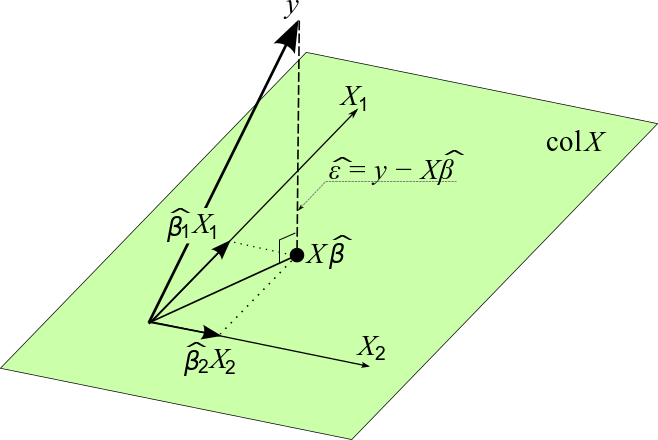
\includegraphics[scale = 0.4]{../images/OLS_geometric_interpretation.png}
\end{center}
So, a brief description of the figure above:
\begin{itemize}
    \item the plane is the space of the predictions $\mathcal{C}(X)$ indeed it is spanned by the column vectors of $X$ 
    \item the vector $\underline{y}$ is the vector of the label to be predicted
    \item the vector $X\hat{\beta}$ in the figure is our prediction $\hat{\underline{y}}$ and correspond to the projection of $\underline{y}$ on the plane $\mathcal{C}(X)$
    \item $\epsilon$ is the residual vector $\underline{r}(\underline{w})$ and represent the error between the predicted value and the actual label
\end{itemize}
If we pick $\underline{\overline{y}} \in \mathcal{C}(X)$ different from $\hat{\underline{y}}$ and their respective residuals: $\underline{\overline{r}} = \underline{y} - \underline{\overline{y}}$ and $\underline{\hat{r}} = \underline{y} - \underline{\hat{y}}$ we have that:
\[
    ||\underline{\hat{r}}||_2 \leq ||\underline{\overline{r}}||_2
\]
Indeed, $\underline{\hat{r}}$ is the orthogonal projection of $\underline{y}$ on $\mathcal{C}(X)$ and the orthogonal projection is the closest point to the vector $\underline{y}$ in the subspace $\mathcal{C}(X)$.\\
Because of this, we can also say that:
\[
    \underline{x_j^\intercal}\underline{\hat{r}} = 0 \hspace{0.5cm} j = 1, \dots, p    
\]
in matrix form:
\[
    X^\intercal \underline{\hat{r}} = \underline{0}   \implies X^\intercal (\underline{y} - \underline{\hat{y}}) = \underline{0} \implies X^\intercal (\underline{y} - X\underline{\hat{w}}) = \underline{0} \implies X^\intercal \underline{y} = X^\intercal X \underline{\hat{w}}
\]
In general the rank of the matrix $X^\intercal X$ is the same as the rank of $X$ so if $X$ is full rank then also $X^\intercal X$ is full rank and this imply that is invertible and we can find $\hat{\underline{w}}$ like this:
\[
    \hat{\underline{w}} = (X^\intercal X)^{-1}X^\intercal \underline{y}
\]
If we are using this linear model for a binary classification we have to apply to the predicted value $\hat{\underline{y}}$ a sign function in order to have the output restrained to \{-1,1\}.\\

\subsection{Optimization}
Here we exploit mathematics for solving the initial problem:
\[
    \hat{\underline{w}} = \underset{\underline{w}}{\arg\min}||\underline{r}(\underline{w})||^2_2 = \underset{\underline{w}}{\arg\min}||\underline{y} - X\underline{w}||^2_2 = \underset{\underline{w}}{\arg\min}(\underline{y} - X\underline{w})^\intercal(\underline{y} - X\underline{w}) =     
\]
\[
    = \underset{\underline{w}}{\arg\min} \bigg[\underline{y}^\intercal \underline{y} - (X\underline{w})^\intercal \underline{y} - \underline{y}^\intercal (X\underline{w}) + (X\underline{w})^\intercal X\underline{w}  \bigg]= \underset{\underline{w}}{\arg\min} \underbrace{\bigg[\underline{y}^\intercal \underline{y} - 2\underline{y}^\intercal X\underline{w} + \underline{w}^\intercal X^\intercal X\underline{w}\bigg]}_{F(\underline{w})}
\]
$F(\underline{w})$ is a \textbf{quadratic functional}. $X$ is full rank, $X^\intercal X$ is positive definite so this means that the functional is strictly convex and has a unique minimum.
So we can compute the gradient and set it to zero:
\[
    \nabla_{\underline{w}}F(\underline{w}) = -2X^\intercal \underline{y} + 2X^\intercal X\underline{w} = \underline{0}
\]
\textbf{Example 1 - Derivation}
\[
    F(\underline{w}) = \underline{w}^\intercal \underline{c} = w_1 c_1 + w_2 c_2 + w_3 c_3 = \underline{c}\underline{w}^\intercal \hspace{1cm} \underline{w}, \underline{c} \in \mathbb{R}^3    
\]
The gradient is:
\[
    \nabla F = \begin{bmatrix}
        \dfrac{\partial F}{\partial w_1}\\
        \dfrac{\partial F}{\partial w_2}\\
        \dfrac{\partial F}{\partial w_3}
    \end{bmatrix} = \begin{bmatrix}
        c_1\\
        c_2\\
        c_3
    \end{bmatrix} = \underline{c}    
\]
\textbf{Example 2 - Derivation}
\[
    F(\underline{w}) = \underline{w}^\intercal A \underline{w} = \sum_{i=1}^n \sum_{j=1}^n w_j a_{ij} w_i \hspace{1cm} A \in \mathbb{R}^{n \times n}    
\]
\[
    \dfrac{\partial}{\partial w_k}(w_j a_{ij} w_i) = \begin{cases}
        a_{ij}w_i & k=j\neq i\\
        w_j a_{ij} & k=i\neq j\\
        0 & k\neq i , k\neq j\\
        2w_k a_{ij} & k=i=j
    \end{cases}    
\]


In the last lecture we have introduced the least squares method. In particular we have mentioned the linear model for which:
\[
    \hat{\underline{y}} = X\hat{\underline{w}} \hspace{1cm} X \in \mathbb{R}^{n \times p} \hspace{0.4cm} \underline{\hat{y}} \in \mathbb{R}^n \hspace{0.4cm} n \geq p \hspace{0.4cm} X \text{ full rank}
\]
We have obtained:
\[
    \underline{\hat{w}} = (X^\intercal X)^{-1} X^\intercal \underline{y} \implies \underline{\hat{y}} = \underbrace{X(X^\intercal X)^{-1} X^\intercal}_{P_x} \underline{y}     
\]
The matrix $P_x$ dimension is given by the product of: $(n\times p)(p\times p)(p \times n) = (n\times n)$ and has this properties:
\begin{itemize}
    \item $P_x = P_x^2$
    \item $P_x$ is a projection matrix
\end{itemize}

Let's consider $U$ an orthogonal ($U^\intercal U = I$) matrix that contains the basis for $\mathcal{C}(X)$ this means that $\mathcal{C}(X) = \mathcal{C}(U)$. We can write:
\[
    \underline{\hat{y}} = X\underline{\hat{w}} = U\underline{\tilde{w}}    
\]
So this basically means that the predicted value of $y$ still a projection on a plane but this time the plane is spanned by the columns of $U$ and not by the columns of $X$. By substituting last equation in the minimization method for least squares we have:
\[
    \underline{\tilde{w}} = \underset{\underline{w}}{\arg\min} ||\underline{y} - U\underline{w}||^2_2 \implies \underline{\hat{y}} = U\underline{\tilde{w}} = U(U^\intercal U)^{-1}U^\intercal \underline{y} = UU^\intercal \underline{y} 
\]
This formulation is possible because this time in the parenthesis we have an orthogonal matrix and this means that $(U^\intercal U)^{-1} = U^\intercal U = I$. In general $UU^\intercal \neq I$ because it might be rectangular (while $U^\intercal U$ is always square).\\

\textbf{Example of usage of U}
We start from $X$:
\[
    X= \begin{bmatrix}
        1& 1 \\
        1 & 3\\
        0 & 0
    \end{bmatrix}
    \hspace{1cm}
    \underline{x_1} = \begin{bmatrix}
        1\\
        1\\
        0   
    \end{bmatrix}
    \hspace{1cm}
    \underline{x_2} = \begin{bmatrix}
        1\\
        3\\
        0
    \end{bmatrix}
\]
How do we build the orthogonal matrix $U$? We can use the Gram-Schmidt procedure:
\[
    \underline{u_1} = \dfrac{\underline{x_1}}{||\underline{x_1}||} = \begin{bmatrix}
        \dfrac{1}{\sqrt{2}}\\
        \dfrac{1}{\sqrt{2}}\\
        0
    \end{bmatrix}    
\]
\[
    \underline{{x'}_2} = \underline{x_2} - (\underline{x_2}^\intercal \underline{u_1})\underline{u_1} = \underline{x_2} - (\underline{u_1^\intercal} \underline{u_1})\underline{x_2} \implies 
    \underline{u_2} = \dfrac{\underline{{x'}_2}}{||\underline{{x'}_2}||} 
    = \begin{bmatrix}
        -\dfrac{1}{\sqrt{2}}\\
        \dfrac{1}{\sqrt{2}}\\
        0
    \end{bmatrix}    
\]
So, the overall matrix $U$ is:
\[
    U = \begin{bmatrix}
        \dfrac{1}{\sqrt{2}} & \dfrac{1}{\sqrt{2}}\\
        -\dfrac{1}{\sqrt{2}} & \dfrac{1}{\sqrt{2}}\\
        0 & 0
    \end{bmatrix}    \hspace{1cm}
    U^\intercal U = I \text{ and } UU^\intercal \neq I
\]
A drawback of Gram Schmidt is that, depending on the order chosen for the columns of $X$, the matrix $U$ can be different. Moreover, the order of vector columns of $U$ is meaningless. \\

Now, we want to exploit the SVD for computing the orthogonal matrix $U$. We start from the SVD of $X$:
\[
    X = U\Sigma V^\intercal    
\]
So
\begin{multicols}{2}
    \[
    \begin{split}
        \underline{\hat{w}} &= (X^\intercal X)^{-1} X^\intercal y\\
        & = (V\Sigma^\intercal U^\intercal U\Sigma V^\intercal)^{-1} V\Sigma^\intercal U^\intercal \underline{y} \\
        & = (V\Sigma^\intercal \Sigma V^\intercal)^{-1} V\Sigma^\intercal U^\intercal \underline{y}\\
        & = V(V\Sigma^\intercal \Sigma V^\intercal)^{-1} V\Sigma^\intercal U^\intercal \underline{y}\\
        & = V(\Sigma^\intercal \Sigma)^{-1} \underbrace{V^\intercal V}_{I}\Sigma^\intercal U^\intercal \underline{y}\\
        & = V\underbrace{(\Sigma^\intercal \Sigma)^{-1} \Sigma^\intercal}_{\Sigma^+} U^\intercal \underline{y}\\ 
        & = V\Sigma^+ U^\intercal \underline{y}
    \end{split}
\]
Recall that:
\[
(AB)^{-1} = B^{-1} A^{-1}    
\]
\[
(V^\intercal)^{-1} = V     
\]
Because $V$ is orthogonal.\\
$\Sigma^+$ il called the pseudo-inverse of $\Sigma$.
\end{multicols}
Eventually, we have:
\[
    \begin{split}
        \underline{\hat{y}} &= X(X^\intercal X)^{-1} X^\intercal \underline{y} = XX^+ \underline{y}\\ 
        &= U(U^\intercal U)^{-1} U^\intercal \underline{y} = UU^+ \underline{y}
    \end{split}
\]
Recalling that we are considering the case in which $n \geq p$, the matrices have these dimensions: $U = (n \times n), \Sigma = (n \times p), V^\intercal = (p \times p)$ and:
\[
    \Sigma = \begin{bmatrix}
        \sigma_1 & 0 & \dots & 0\\
        0 & \sigma_2 & \dots & 0\\
        \vdots & \vdots & \ddots & \vdots\\
        0 & 0 & \dots & \sigma_p\\
        0 & 0 & \dots & 0\\
        \vdots & \vdots & \ddots & \vdots\\
        0 & 0 & \dots & 0
    \end{bmatrix}
\]
\[
    \Sigma^\intercal \Sigma = \begin{bmatrix}
        \sigma_1 & 0 & \dots & 0 & 0 & \dots & 0\\
        0 & \sigma_2 & \dots & 0 & 0 & \dots & 0\\
        \vdots & \vdots & \ddots & \vdots & \vdots & \ddots & \vdots\\
        0 & 0 & \dots & \sigma_p & 0 & \dots & 0
    \end{bmatrix} 
    \begin{bmatrix}
        \sigma_1 & 0 & \dots & 0\\
        0 & \sigma_2 & \dots & 0\\
        \vdots & \vdots & \ddots & \vdots\\
        0 & 0 & \dots & \sigma_p\\
        0 & 0 & \dots & 0\\
        \vdots & \vdots & \ddots & \vdots\\
        0 & 0 & \dots & 0
    \end{bmatrix}
    =
    \begin{bmatrix}
        \sigma_1^2 & 0 & \dots & 0\\
        0 & \sigma_2^2 & \dots & 0\\
        \vdots & \vdots & \ddots & \vdots\\
        0 & 0 & \dots & \sigma_p^2\\
    \end{bmatrix}
\]
\[
    (\Sigma^\intercal \Sigma)^{-1} = \begin{bmatrix}
        \dfrac{1}{\sigma_1^2} & 0 & \dots & 0\\
        0 & \dfrac{1}{\sigma_2^2} & \dots & 0\\
        \vdots & \vdots & \ddots & \vdots\\
        0 & 0 & \dots & \dfrac{1}{\sigma_p^2}\\
    \end{bmatrix}    
\]
\[
    \Sigma^+ =  (\Sigma^\intercal \Sigma)^{-1} \Sigma^\intercal = \begin{bmatrix}
        \dfrac{1}{\sigma_1} & 0 & \dots & 0 & 0 & \dots & 0\\
        0 & \dfrac{1}{\sigma_2} & \dots & 0 & 0 & \dots & 0\\
        \vdots & \vdots & \ddots & \vdots & \vdots & \ddots & \vdots\\
        0 & 0 & \dots & \dfrac{1}{\sigma_p} & 0 & \dots & 0
    \end{bmatrix}
\]

Let's consider now the case in which $p \geq n$ and $X$ has $n$ linearly independent rows (before we had $p$ linearly independent columns). This means that we have more unknowns than equations and we would find infinite solutions for $\underline{\hat{w}}$ such that $\underline{\hat{y}} = X\underline{\hat{w}}$. 

The solution found before $\underline{\hat{w}} = V\Sigma^+ U^\intercal \underline{y}$ it's still valid but now $\Sigma^+ = \Sigma^\intercal(\Sigma\Sigma^\intercal)^{-1}$ so it has the same shape as before but transposed. 
Summary:
\begin{multicols}{2}
    \begin{center}
        $n > p$\\
        \vspace{0.3cm}
        \begin{tikzpicture}
            \draw (-1,0) -- (1,0) -- (1,4) -- (-1,4) -- (-1,0) -- (0,0) node[below]{$n$};
            \draw (1,0) -- (1,2) node[right]{$p$};
        \end{tikzpicture}
        \[
            \underline{\hat{w}} = V\Sigma^+ U^\intercal \underline{y}    
        \]
        \[
            \Sigma^+ = (\Sigma^\intercal \Sigma)^{-1} \Sigma^\intercal
        \]
    \end{center}
    \newcolumn
    \begin{center}
        $p > n$\\
        \vspace{0.3cm}
        \begin{tikzpicture}
            \draw (-2,0) -- (2,0) -- (2,2) -- (-2,2) -- (-2,0) -- (0,0) node[below]{$p$};
            \draw (2,0) -- (2,1) node[right]{$n$};
        \end{tikzpicture}
        \[
            \underline{\hat{w}} = V\Sigma^+ U^\intercal \underline{y}    
        \]
        \[
            \Sigma^+ = \Sigma^\intercal(\Sigma\Sigma^\intercal)^{-1}    
        \]

    \end{center}
\end{multicols}


Let's recap what we have seen so far regarding the Least Squares method.
\[
    (x_i, y_i) \hspace{0.2cm} i = 1, \dots, n  \hspace{1cm} \underline{x_i} \in \mathbb{R}^p \text{ and } y_i \in \mathbb{R}
\]
In matrix form:
\[
    X \in \mathbb{R}^{n \times p} \text{ and } \underline{y} \in \mathbb{R}^n    
\]
We have made the hypothesis, until now, of having a full rank matrix $X$. The linear model is defined as:
\[
    \underline{\hat{y}} = X\underline{\hat{w}}_{LS} \hspace{1cm} \text{with} \hspace{1cm} \underline{\hat{w}}_{LS} = (X^\intercal X)^{-1} X^\intercal \underline{y}    
\]
Moreover, we said that the actual value of $y$ is not exactly given by this linear model but it will be an approximation:
\[
    y \approx X \underline{w}_{LS}
\]
And this can be written by expliciting an error:
\[
    \underline{y} = X\underline{w}^* + \underline{\epsilon}    
\]
where $\underline{\epsilon}$ is the error or noise vector. If we replace this last equation in the one with $\underline{\hat{w}}_{LS}$ we get:
\[
    \underline{\hat{w}}_{LS} = (X^\intercal X)^{-1} X^\intercal (X\underline{w}^* + \underline{\epsilon}) = \underline{w}^* + (X^\intercal X)^{-1} X^\intercal \underline{\epsilon} =      
\]
Now we can apply the SVD to $X$ so, if we call $X = U\Sigma V^\intercal$ we get, from previous lectures, that: $(X^\intercal X)^{-1} X^\intercal = V\Sigma^+ U^\intercal$. We have said before that $X$ is full rank so we will have all singular components different than 0 and $\sigma_1 > \sigma_2 > \dots > \sigma_p > 0$. The matrix $\Sigma^+$ is a psuedo-diagonal matrix with the inverse of the singular values on the diagonal (check few pages above). 
\[
    =  \underline{w}^* + V\Sigma^+ U^\intercal \underline{\epsilon}    
\]
\begin{itemize}
    \item $U^\intercal \underline{\epsilon}$: we multiply a vector with an orthogonal matrix so its norm will not change.
    \item $V\Sigma^+ U^\intercal \underline{\epsilon}$: we multiply a vector with a diagonal matrix so we will have a scaling of the vector. But \textbf{if a singular value is very very small, its inverse in the matrix SigmaPlus will be huge and will scale the error vector a lot! So the error will be amplified and the original model vector w* will be negligible}.
\end{itemize}

\subsection{Ridge regression (regularization)}
This method will help us in preventing the problem mentioned just before. We start from the definition of the weight vector for linear model explicited for the optimization method of the Least Squares:
\[
    \underline{\hat{w}}_{LS} = \arg \min_{\underline{w}} \underbrace{||\underline{y} - X\underline{w}||_2^2 + \lambda ||\underline{w}||_2^2}_{f(\underline{w})}
\]
In particular we have added a term. 
\[
    f(\underline{w}) = \underline{y}^\intercal \underline{y} - 2\underline{w}^\intercal X \underline{y} + \underline{w}^\intercal X^\intercal X \underline{w} + \lambda \underline{w}^\intercal \underline{w}
\]
We can now compute the gradient of this function:
\[
        \nabla_w(f(\underline{w})) = -2X^\intercal \underline{y} + 2X^\intercal X \underline{w} + 2\lambda \underline{w} = 0      
\]
\[
    X^\intercal \underline{y} = (X^\intercal X + \lambda I)\underline{w}     
\]
\[
    \underline{\hat{w}}_{R} = (X^\intercal X + \lambda I)^{-1} X^\intercal \underline{y}    
\]
It's easy to notice that if $\lambda = 0$ we get the Least Squares solution. If $\lambda > 0$ we will have a different solution. We can now compute the SVD of $X$:
\[
    \begin{split}
        \underline{\hat{w}}_R &= (V\Sigma^\intercal \underbrace{U^\intercal U}_{I} \Sigma V^\intercal + \lambda \underbrace{V^\intercal V}_{I})^{-1} V\Sigma^\intercal U^\intercal \underline{y} \\
        &= \left[V(\Sigma^\intercal \Sigma + \lambda I)V^\intercal\right]^{-1} V\Sigma^\intercal U^\intercal \underline{y} \\
        &= V\underbrace{(\Sigma^\intercal \Sigma + \lambda I) \Sigma^\intercal}_{M}U^\intercal \underline{y} \\
    \end{split}    
\]
Where 
\[
M = \begin{bmatrix}
    \dfrac{\sigma_1}{\sigma_1^2 + \lambda} & 0 & \dots & 0 & 0 & \dots & 0\\
    0 & \dfrac{\sigma_2}{\sigma_2^2 + \lambda} & \dots & 0 & 0 & \dots & 0\\
    \vdots & \vdots & \ddots & \vdots & \vdots & \ddots & \vdots\\
    0 & 0 & \dots & \dfrac{\sigma_p}{\sigma_p^2 + \lambda} & 0 & \dots & 0
\end{bmatrix}
\]
\begin{itemize}
    \item if $\sigma_i$ is big compared to $\lambda$ then $\dfrac{\sigma_i}{\sigma_i^2 + \lambda} \approx \dfrac{1}{\sigma_i}$
    \item if $\sigma_i$ is close to 0 then $\dfrac{\sigma_i}{\sigma_i^2 + \lambda} \approx 0$
\end{itemize}
If we now consider again the problem of having a singular value close to 0 we can see that it is now solved because we would reconduct to the second case just above and the pseudo inverse would be almost 0. 
If $\lambda$ is very small the matrix of $\Sigma$'s is almost equal to $\Sigma^+$.
\[
    \begin{split}
        \underline{\hat{w}}_R &= (X^\intercal X + \lambda I)^{-1} X^\intercal \underline{y}\\
        &= (X^\intercal X + \lambda I)^{-1} X^\intercal(X\underline{w}^* + \underline{\epsilon})\\
        &= (X^\intercal X + \lambda I)^{-1} X^\intercal X\underline{w}^* + (X^\intercal X + \lambda I)^{-1} X^\intercal \underline{\epsilon}\\
    \end{split}    
\]
If $\underline{\epsilon} = \underline{0}$ then there is only the first term and, since we are not finding the perfect projection on the plane, we make an higher error with respect to Least Squares. 

\section{Page Rank}
Consider 4 websites, the arrows represents the link from one site to another. 
\begin{multicols}{2}
    \begin{center}
        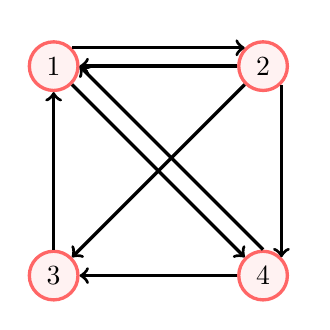
\begin{tikzpicture}[
        SIR/.style={circle, draw=red!60, fill=red!5, very thick, minimum size=5mm},
        node distance=2cm
        ]
        %Nodes
        \node[SIR]    (1)                              {1};
        \node[SIR]    (2)       [right=of 1] {2};
        \node[SIR]    (3)       [below=of 1] {3};
        \node[SIR]    (4)       [right=of 3] {4};
        
        %Lines
        \draw[->, very thick] (1.north east)  to node[above right] { } (2.north west);
        \draw[->, very thick] (1.south east)  to node[below right, sloped] { } (4.north west);
        \draw[->, very thick] (2.south east)  to node[right] { } (4.north east);
        \draw[->, very thick] (2.west)  to node[below right] { } (1.east);
        \draw[->, very thick] (3.north)  to node[right] { } (1.south);
        \draw[->, very thick] (2.south west)  to node[above left, sloped] { } (3.north east);
        \draw[->, very thick] (4.west)  to node[above right] { } (3.east);
        \draw[->, very thick] (4.north)  to node[above right, sloped] { } (1.east);
        \end{tikzpicture}
    \end{center}
    
The idea is to surf the web randomly (random walks on the graph) and if you do that long enough you will reach a \textbf{Steady state} where $\pi_i$ will be the probability of being on the i-th website.\\
In this case the vector $\underline{\pi} \in \mathbb{R}^4$ because there are 4 websites. 
\end{multicols}
We are assuming there are not separated sites. How can we represent the matrix? It an \textbf{Adjacency matrix}
\[
    \tilde{A} = \begin{bmatrix}
        0 & 1 & 1 & 1\\
        0 & 0 & 1 & 1\\
        1 & 0 & 0 & 0\\
        1 & 0 & 1 & 0\\
    \end{bmatrix}
    \rightarrow
    \tilde{A}_{ij} = \begin{cases}
        1 & \text{if there is a link from i to j}\\
        0 & \text{otherwise}
    \end{cases}    
    \hspace{0.5cm}
    \overset{\text{normalized version}}{\longrightarrow}
    A = \begin{bmatrix}
        0   & 1 & 1/3 & 1/2\\
        0   & 0 & 1/3 & 1/2\\
        1/2 & 0 & 0   & 0\\
        1/2 & 0 & 1/3 & 0\\
    \end{bmatrix}
\]
In the normalized version all columns sum up to 1. What happen if we multiply the matrix $A$ times a canonical basis vector $\underline{e}_3 = \begin{bmatrix}
    0 & 0 & 1 & 0
\end{bmatrix}^\intercal$?
\[
    A\underline{e_3} = \begin{bmatrix}
        1/3\\
        1/3\\
        0\\
        1/3\\
    \end{bmatrix}
\]
As it was trivial to figure, we obtain, in this case, the third column of the adjacency matrix. In a probability perspective, the vector $\underline{e}_3$ represents the probability of starting from the third website. The vector we obtain is the probability of reaching the other websites starting from the third one. This means that in this case we are certain that we start from the third website and for sure we won't be in that site in the following iteration. \\

Considering 
\[
\underline{\pi} = \begin{bmatrix}
    \pi_1\\
    \pi_2\\
    \pi_3\\
    \pi_4\\
\end{bmatrix}    
\]
The steady state is defined as: $A\underline{\pi} = \underline{\pi}$.
This means that, the steady state is the eigenvector of the matrix $A$ with eigenvalue 1. The matrix $A$ is positive (not positive-definite) i.e. it has all non-negative cohefficients. A positive matrix is denoted with $A > 0$.
From Perron-Frobenius theory we know that $\lambda_1 = 1$ is the largest eigenvalue.
\[
    \lambda_1 = 1 > \lambda_2 > \lambda_3 > \dots > \lambda_n \hspace{1cm} \lambda_i \neq 0
\] 
As mentioned in a previous lecture, we can use the power method in order to retrieve the largest eigenvalue. In particular, we start from:
\[
    \underline{\pi}^{(0)} \hspace{0.5cm}\text{with}\hspace{0.5cm} ||\underline{\pi}^{(0)}||=1    
\]
Then, for $k = 1, 2, \dots $
\[
    \underline{\pi}^{(k)} = \dfrac{A\underline{\pi}^{(k-1)}}{||A\underline{\pi}^{(k-1)}||}    
\]
\[
    \text{if } ||\underline{\pi}^{(k)} - \underline{\pi}^{(k-1)}|| < \epsilon \text{ then stop}    
\]
Obviously, $\epsilon$ represents a tolerance value. As we can see, there is an recursive definition in a sense that, at each iteration, the same operation is made on the same variable. For example:
\[
    \underline{\pi}^{(1)} = \dfrac{A\underline{\pi}^{(0)}}{||A\underline{\pi}^{(0)}||}    
    \hspace{2cm}
    \underline{\pi}^{(2)} = \dfrac{A\underline{\pi}^{(1)}}{||A\underline{\pi}^{(1)}||} = \dfrac{A^2\underline{\pi}^{()}}{||A^2\underline{\pi}^{(k-1)}||} 
\]
So, iterating k times:
\[
    \underline{\pi}^{(k)} = \dfrac{A^k\underline{\pi}^{(0)}}{||A^k\underline{\pi}^{(0)}||}     
\]
Since in $A$ there are no columns that are completely equal to 0, the matrix can be diagonalized. This implies that there are some $\underline{v}_i, i = 1, \dots, n$ that can used as a basis for the space. In particular we can write:
\[
    \underline{\pi}^{(0)} = \sum_{i=1}^n \alpha_i \underline{v}_i
\]
We want to plug this expression in the previous equation (power method). Before, notice that, $A\underline{v}_i = \lambda \underline{v}_i$ because $\underline{v}_i$ are the vectors which diagonalize $A$ so the ones such that $A = V\Lambda V^\intercal$. 
The numerator of $\underline{\pi}^{(k)}$ can be written as:
\[
    A^k \underline{\pi}^{(0)} = \alpha_1\lambda_1^k \left(\underline{v}_1 + \sum_{i=2}^{n} \dfrac{\alpha_i}{\alpha_1}\left(\dfrac{\lambda_i}{\lambda_1}\right)^k \underline{v}_i\right)    
\]
Proof:
\begin{multicols}{2}
    \[
    \begin{split}
        A^k \underline{\pi}^{(0)} &= V\Lambda^k V^{-1} \left(\alpha_1\underline{v}_1 + \dots + \alpha_n\underline{v}_n\right)\\
        &\overset{\circledast }{=} V\Lambda^k \left(\alpha_1\underline{e}_1 + \dots + \alpha_n\underline{e}_n\right)\\
        &= V\left(\alpha_1\lambda_1^k\underline{e}_1 + \dots + \alpha_n\lambda_n^k\underline{e}_n \right)\\
        &\overset{\diamond}{=} \alpha_1\lambda_1^k\underline{v}_1 + \dots + \alpha_n\lambda_n^k\underline{v}_n\\
        &= \alpha_1\lambda_1^k \left(\underline{v}_1 + \dfrac{\alpha_2}{\alpha_1}\left(\dfrac{\lambda_2}{\lambda_1}\right)^k \underline{v}_2 + \dots + \dfrac{\alpha_n}{\alpha_1}\left(\dfrac{\lambda_n}{\lambda_1}\right)^k \underline{v}_n\right)\\
    \end{split}
\]
\[
    \circledast  \rightarrow V^{-1}\underline{v}_i = V^{-1}\underline{v}_i = \begin{bmatrix}
        \horzbar & \underline{v}_1^\intercal & \horzbar\\
        \horzbar & \underline{v}_2^\intercal & \horzbar\\    
         & \vdots & \\
        \horzbar & \underline{v}_n^\intercal & \horzbar
    \end{bmatrix} \underline{v}_i
    = \underline{e}_i
\]
\[
    \diamond \rightarrow A\underline{v} = \lambda\underline{v} \implies AA\underline{v} = \lambda A\underline{v} \implies A^2\underline{v} = \lambda^2\underline{v}     
\]
\end{multicols}
If $k \to \infty$ then $\left(\dfrac{\lambda_i}{\lambda_1}\right)^k \to 0$ because $\lambda_1 > \lambda_i$ for $i = 2, \dots, n$ . So, the only remaining term is $\underline{v}_1$ which is the eigenvector with the largest eigenvalue. So what we have just done is the proof of the convergence of the power method.The closer are the eigenvalues to $\lambda_1$ the slower is the convergence.

   % lecture 8 absent because it was a lab
So far we have considered:
\[
    \underline{y} = X\underline{w} \hspace{1cm} X \in \mathbb{R}^{n \times p} \text{ and } \begin{Bmatrix}
        \text{Least Squares}: \underline{\hat{w}}_LS\\
        \text{Ridge Regression}: \underline{\hat{w}}_{RR}\\
    \end{Bmatrix} \underline{w} \in \mathbb{R}^p \text{ dense vector, i.e. not many zeros} 
\]
We are going to see a method which obtain a vector $\underline{\hat{w}}$ with many zeros, as sparse as possible. We want to consider this model:
\[
    \underline{y} = X\underline{w} \hspace{1cm} X \in \mathbb{R}^{n \times p} \hspace{1cm} p > n 
\]
We have said that the system is undetermined since it has infinite solutions. Suppose to have 2 features and 1 sample. 
\[
    X = \begin{bmatrix}
        2 & 3\\
    \end{bmatrix}
    \hspace{1cm}
    y = \begin{bmatrix}
        1\\
    \end{bmatrix}
\]
And so:
\[
    1 = \begin{bmatrix}
        2 & 3
    \end{bmatrix}\begin{bmatrix}
        w_1\\
        w_2
    \end{bmatrix} \implies
    1 = 2w_1 + 3w_2 \hspace{0.2cm} \leftarrow \hspace{0.2cm} \text{line}    
\]
As mentioned in a previous lecture, we want to find the minimum length solution so we can plot the line found before and the circles that represents the l2-norm distance.
\begin{center}
    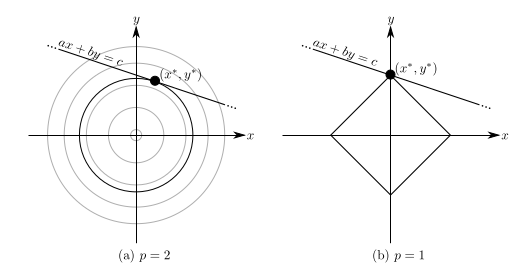
\includegraphics[scale=0.6]{../images/LassoRidgePlot.png}
\end{center}
On the right-hand side it is represented the equivalent plot but with the l1-norm. We can see that the solution on the right has one coordinate (are features!) that is equal to zero. This is true in general, i.e. we will obtain sparser solution using the l1-norm rather than the l2-norm.\\
With L1-norm it's still a convex optimization problem and
\[
    F(\underline{w}) = ||X\underline{w} - \underline{y}||_2^2 + \lambda ||\underline{w}||_1    
\] 
This model is implemented by \textbf{Lasso} (Least Absolute Shrinkage and Selection Operator) and achieve both the shortest distance solution and the selection of some features.

This is important because by reducing the number of features, we increase the interpretability of the model.\\

There is also the \textbf{Elastic Net} which combines both Lasso and Ridge: 
\[
    F(\underline{w}) = ||X\underline{w} - \underline{y}||_2^2 + \lambda_1||\underline{w}||_1 + \lambda_2||\underline{w}||_2^2  
\] 

\vspace{2cm}
Once again, we start considering:
\[
    \underline{y} \in \mathbb{R}^n \hspace{1cm} X \in \mathbb{R}^{n \times p} \hspace{0.2cm} \text{with \emph{p} lin. ind. cols } (\implies \sigma_i > 0, \hspace{0.1cm} i = 1, \dots, p)  
\]
Now we write the formulation of the weights vector $w$ we found for Ridge Regression. 
\[
    \begin{split}
    \underline{\hat{w}}_R &= V\underbrace{(\Sigma^\intercal \Sigma + \lambda I)^{-1} \Sigma^\intercal}_{\substack{\Sigma^\intercal(\Sigma \Sigma^\intercal + \lambda I)^{-1}}} U^\intercal \underline{y}\\
    &= \underbrace{V\Sigma^\intercal U^\intercal}_{X^\intercal} \underbrace{U(\Sigma \Sigma^\intercal + \lambda I)^{-1} U^\intercal \underline{y}}_{\underline{\alpha} \in \mathbb{R}^n}\\
    &= X^\intercal \underline{\alpha}\\
    &= \sum_{i=1}^n \alpha_i \underline{x}_i\\
    \end{split}     
\]
In the second passage we have added the matrices $U^\intercal U$ because its the identity matrix. We obtain a weighted sum of the column vectors of $X^\intercal$, where $X$ is:
\[
X = \begin{bmatrix}
    \horzbar & \underline{x_1^\intercal} & \horzbar\\
    \horzbar & \underline{x_2^\intercal} & \horzbar\\    
     & \vdots & \\
    \horzbar & \underline{x_n^\intercal} & \horzbar
\end{bmatrix}
\]
So, until now, we have discussed about linear models. A generic form would be:
\[
    \hat{y}_i = w_1x_{i1} + w_2x_{i2} \hspace{1cm} \text{if} \hspace{1cm} \underline{x}_i = \begin{bmatrix}
        x_{i1}\\
        x_{i2}
    \end{bmatrix}    
\]
Now a new model:
\[
    \hat{y}_i = w_1x_{i1} + w_2x_{i2} + w_3x_{i1}^2 + w_4x_{i2}^2 + w_5x_{i1}x_{i2}    
\]
So, the original feature vector $\underline{x}$ is transformed into a new feature vector by means of function called feature map $\phi(x)$:
\[
    \phi(x) = \begin{bmatrix}
        x_1\\
        x_2\\
        x_1^2\\
        x_2^2\\
        x_1x_2
    \end{bmatrix} \in \mathbb{R}^d \hspace{1cm} d > p \text{ typically}    
\]
And
\[
    \hat{y}_i = \phi(x_i)^\intercal \underline{w}    
\]
In general $d$ can be huge.


\section{Kernel Methods}
The aim of this methods is to avoid the necessity of computing huge vectors.
\[
    \Phi =  \begin{bmatrix}
        \horzbar & \phi(\underline{x}_1)^\intercal & \horzbar\\
        \horzbar & \phi(\underline{x}_2)^\intercal & \horzbar\\    
         & \vdots & \\
        \horzbar & \phi(\underline{x}_n)^\intercal & \horzbar
    \end{bmatrix}
    \in \mathbb{R}^{n \times d} \hspace{1cm} \underline{\hat{y}} = \Phi \underline{w}
\]
The objective is still the same: i.e. finding $\underline{w}$. We are now going to consider ridge regression in order to achieve that. 
Instead of $\underline{\hat{w}}_R = X^\intercal \underline{\alpha}$ we can now write:
\[
    \underline{\hat{w}}_R = \Phi^\intercal \underline{\alpha}
\]
Where
\[
    \underline{\alpha} = U(\Sigma \Sigma^\intercal + \lambda I)^{-1} U^\intercal \underline{y} = (XX^\intercal + \lambda I)^{-1} \underline{y}    
\]
Here is the proof:
\[
    (U\Sigma V^\intercal V\Sigma^\intercal U^\intercal + \lambda UU^\intercal)^{-1} \underline{y}    
\]


\end{document}